\chapter{多元函数微分学}

\section{可 微 性}

\subsection{可微性与全微分}

与一元函数一样, 在多元函数微分学中, 主要讨论多元函数的可微性及其应用. 本章重点建立二元函数可微性概念,至于一般 \(n\) 元函数的可微性不难据此相应地给出 (对此, 在第二十三章有更详细的论述).

%定义  1
\begin{definition}{}{def:}

\end{definition}
设函数 \(z = f\left( {x,y}\right)\) 在点 \({P}_{0}\left( {{x}_{0},{y}_{0}}\right)\) 的某邻域 \(U\left( {P}_{0}\right)\) 上有定义,对于 \(U\left( {P}_{0}\right)\) 中的点 \(P\left( {x,y}\right)  = \left( {{x}_{0} + {\Delta x},{y}_{0} + {\Delta y}}\right)\) ,若函数 \(f\) 在点 \({P}_{0}\) 处的全增量 \({\Delta z}\) 可表示为
\[
{\Delta z} = f\left( {{x}_{0} + {\Delta x},{y}_{0} + {\Delta y}}\right)  - f\left( {{x}_{0},{y}_{0}}\right)
\]
\[
= {A\Delta x} + {B\Delta y} + o\left( \rho \right) , \tag{1}
\]
其中 \(A,B\) 是仅与点 \({P}_{0}\) 有关的常数, \(\rho  = \sqrt{\Delta {x}^{2} + \Delta {y}^{2}},o\left( \rho \right)\) 是较 \(\rho\) 高阶的无穷小量,则称函数 \(f\) 在点 \({P}_{0}\) 可微. 并称 (1) 式中关于 \({\Delta x},{\Delta y}\) 的线性函数 \({A\Delta x} + {B\Delta y}\) 为函数 \(f\) 在点 \({P}_{0}\) 的全微分, 记作
\[
{\left. \mathrm{d}z\right| }_{{P}_{0}} = \mathrm{d}f\left( {{x}_{0},{y}_{0}}\right)  = {A\Delta x} + {B\Delta y}. \tag{2}
\]
由 (1),(2) 可见 \(\mathrm{d}z\) 是 \({\Delta z}\) 的线性主部,特别当 \(\left| {\Delta x}\right| ,\left| {\Delta y}\right|\) 充分小时,全微分 \(\mathrm{d}z\) 可作为全增量 \({\Delta z}\) 的近似值,即
\[
f\left( {x,y}\right)  \approx  f\left( {{x}_{0},{y}_{0}}\right)  + A\left( {x - {x}_{0}}\right)  + B\left( {y - {y}_{0}}\right) . \tag{3}
\]
在使用上, 有时也把 (1) 式写成如下形式:
\[
{\Delta z} = {A\Delta x} + {B\Delta y} + {\alpha \Delta x} + {\beta \Delta y}, \tag{4}
\]
这里
\[
\mathop{\lim }\limits_{{\left( {{\Delta x},{\Delta y}}\right)  \rightarrow  \left( {0,0}\right) }}\alpha  = \mathop{\lim }\limits_{{\left( {{\Delta x},{\Delta y}}\right)  \rightarrow  \left( {0,0}\right) }}\beta  = 0.
\]
%例 1
\begin{example}

\end{example}
考察函数 \(f\left( {x,y}\right)  = {xy}\) 在点 \(\left( {{x}_{0},{y}_{0}}\right)\) 处的可微性.

%解
\begin{solution}

\end{solution}
在点 \(\left( {{x}_{0},{y}_{0}}\right)\) 处函数 \(f\) 的全增量为
\[
{\Delta f}\left( {{x}_{0},{y}_{0}}\right)  = \left( {{x}_{0} + {\Delta x}}\right) \left( {{y}_{0} + {\Delta y}}\right)  - {x}_{0}{y}_{0}
\]
\[
= {y}_{0}{\Delta x} + {x}_{0}{\Delta y} + {\Delta x\Delta y}.
\]
由于
\[
\frac{\left| \Delta x\Delta y\right| }{\rho } = \rho \frac{\left| \Delta x\right| }{\rho }\frac{\left| \Delta y\right| }{\rho } \leq  \rho  \rightarrow  0\;\left( {\rho  \rightarrow  0}\right) ,
\]
因此 \({\Delta x\Delta y} = o\left( \rho \right)\) . 从而函数 \(f\) 在 \(\left( {{x}_{0},{y}_{0}}\right)\) 可微,且
\[
\mathrm{d}f = {y}_{0}{\Delta x} + {x}_{0}{\Delta y}.
\]
\subsection{偏导数}

由一元函数微分学知道: 若 \(f\left( x\right)\) 在点 \({x}_{0}\) 可微,则函数增量 \(f\left( {{x}_{0} + {\Delta x}}\right)  - f\left( {x}_{0}\right)  = {A\Delta x} +\)  \(o\left( {\Delta x}\right)\) ,其中 \(A = {f}^{\prime }\left( {x}_{0}\right)\) . 同样,由上一段已知,若二元函数 \(f\) 在点 \(\left( {{x}_{0},{y}_{0}}\right)\) 可微,则 \(f\) 在 \(\left( {{x}_{0},{y}_{0}}\right)\) 处的全增量可由 (1) 式表示. 现在讨论其中 \(A,B\) 的值与函数 \(f\) 的关系. 为此,在 (4)式中令 \({\Delta y} = 0\left( {{\Delta x} \neq  0}\right)\) ,这时得到 \({\Delta z}\) 关于 \(x\) 的偏增量 \({\Delta }_{x}z\) ,且有
\[
{\Delta }_{x}z = {A\Delta x} + {\alpha \Delta x}\text{ 或 }\frac{{\Delta }_{x}z}{\Delta x} = A + \alpha .
\]
现让 \({\Delta x} \rightarrow  0\) ,由上式便得 \(A\) 的一个极限表示式
\[
A = \mathop{\lim }\limits_{{{\Delta x} \rightarrow  0}}\frac{{\Delta }_{x}z}{\Delta x} = \mathop{\lim }\limits_{{{\Delta x} \rightarrow  0}}\frac{f\left( {{x}_{0} + {\Delta x},{y}_{0}}\right)  - f\left( {{x}_{0},{y}_{0}}\right) }{\Delta x}. \tag{5}
\]
容易看出,(5)式右边的极限正是关于 \(x\) 的一元函数 \(f\left( {x,{y}_{0}}\right)\) 在 \(x = {x}_{0}\) 处的导数. 类似地,令 \({\Delta x} = 0\left( {{\Delta y} \neq  0}\right)\) ,由 (4) 式又可得到
\[
B = \mathop{\lim }\limits_{{{\Delta y} \rightarrow  0}}\frac{{\Delta }_{y}z}{\Delta y} = \mathop{\lim }\limits_{{{\Delta y} \rightarrow  0}}\frac{f\left( {{x}_{0},{y}_{0} + {\Delta y}}\right)  - f\left( {{x}_{0},{y}_{0}}\right) }{\Delta y}. \tag{6}
\]
它是关于 \(y\) 的一元函数 \(f\left( {{x}_{0},y}\right)\) 在 \(y = {y}_{0}\) 处的导数.

二元函数当固定其中一个自变量时, 它对另一个自变量的导数称为偏导数, 定义如下.

%定义  2
\begin{definition}{}{def:}

\end{definition}
设函数 \(z = f\left( {x,y}\right) ,\left( {x,y}\right)  \in  D\) . 若 \(\left( {{x}_{0},{y}_{0}}\right)  \in  D\) ,且 \(f\left( {x,{y}_{0}}\right)\) 在 \({x}_{0}\) 的某邻域内有定义, 则当极限
\[
\mathop{\lim }\limits_{{{\Delta x} \rightarrow  0}}\frac{{\Delta }_{x}f\left( {{x}_{0},{y}_{0}}\right) }{\Delta x} = \mathop{\lim }\limits_{{{\Delta x} \rightarrow  0}}\frac{f\left( {{x}_{0} + {\Delta x},{y}_{0}}\right)  - f\left( {{x}_{0},{y}_{0}}\right) }{\Delta x} \tag{7}
\]
存在时,称这个极限为函数 \(f\) 在点 \(\left( {{x}_{0},{y}_{0}}\right)\) 关于 \(x\) 的偏导数,记作
\[
{f}_{x}\left( {{x}_{0},{y}_{0}}\right) \text{ 或 }{z}_{x}\left( {{x}_{0},{y}_{0}}\right) ,{\left. \frac{\partial f}{\partial x}\right| }_{\left( {x}_{0},{y}_{0}\right) },{\left. \frac{\partial z}{\partial x}\right| }_{\left( {x}_{0},{y}_{0}\right) }.
\]
同样定义 \(f\) 在点 \(\left( {{x}_{0},{y}_{0}}\right)\) 关于 \(y\) 的偏导数 \({f}_{y}\left( {{x}_{0},{y}_{0}}\right)\) 或 \({\left. \frac{\partial f}{\partial y}\right| }_{\left( {x}_{0},{y}_{0}\right) }\) .

%注
\begin{remark}

\end{remark}
1 这里符号 \(\frac{\partial }{\partial x},\frac{\partial }{\partial y}\) 专用于偏导数算符,与一元函数的导数符号 \(\frac{\mathrm{d}}{\mathrm{d}x}\) 相仿,但又有差别.

%注
\begin{remark}

\end{remark}
2 在上述定义中, \(f\) 在点 \(\left( {{x}_{0},{y}_{0}}\right)\) 存在关于 \(x\left( {\text{ 或 }y}\right)\) 的偏导数, \(f\) 至少在 \(\{ (x\) , \(\left. {y)\left| {y = {y}_{0},}\right| x - {x}_{0} \mid   < \delta }\right\}\) (或 \(\left\{  {\left( {x,y}\right) \left| {x = {x}_{0},}\right| y - {y}_{0} \mid   < \delta }\right\}\) ) 上必须有定义.

若函数 \(z = f\left( {x,y}\right)\) 在区域 \(D\) 上每一点(x, y)都存在对 \(x\) (或对 \(y\) ) 的偏导数,则得到函数 \(z = f\left( {x,y}\right)\) 在区域 \(D\) 上对 \(x\) (或对 \(y\) ) 的偏导函数 (也简称偏导数),记作
\[
{f}_{x}\left( {x,y}\right) \text{ 或 }\frac{\partial f\left( {x,y}\right) }{\partial x}\;\left( {{f}_{y}\left( {x,y}\right) \text{ 或 }\frac{\partial f\left( {x,y}\right) }{\partial y}}\right) ,
\]
也可简单地写作 \({f}_{x},{z}_{x}\) 或 \(\frac{\partial f}{\partial x},\frac{\partial z}{\partial x}\left( {{f}_{y},{z}_{y}}\right.\) 或 \(\left. {\frac{\partial f}{\partial y},\frac{\partial z}{\partial y}}\right)\) .

在上一章中已指出,二元函数 \(z = f\left( {x,y}\right)\) 的几何图像通常是三维空间中的曲面. 设 \({P}_{0}\left( {{x}_{0},{y}_{0},{z}_{0}}\right)\) 为这曲面上一点,其中 \({z}_{0} = f\left( {{x}_{0},{y}_{0}}\right)\) . 过 \({P}_{0}\) 作平面 \(y = {y}_{0}\) ,它与曲面 \(z = f\left( {x,y}\right)\) 的交线
\[
C : \left\{  \begin{array}{l} y = {y}_{0}, \\  z = f\left( {x,y}\right)  \end{array}\right.
\]
是平面 \(y = {y}_{0}\) 上的一条曲线. 于是,二元函数偏导数的几何意义 (如图 17-1) 是: \({f}_{x}\left( {{x}_{0},{y}_{0}}\right)\) 作为一元函数 \(f\left( {x,{y}_{0}}\right)\) 在 \(x = {x}_{0}\) 的导数,就是曲线 \(C\) 在点 \({P}_{0}\) 处的切线 \({T}_{x}\) 对于 \(x\) 轴的斜率,即 \({T}_{x}\) 与 \(x\) 轴正向所成倾角的正切 \(\tan \alpha\) . 同样, \({f}_{y}\left( {{x}_{0},{y}_{0}}\right)\) 是平面 \(x = {x}_{0}\) 与曲面 \(z = f\left( {x,y}\right)\) 的交线
\[
\left\{  \begin{array}{l} x = {x}_{0}, \\  z = f\left( {x,y}\right)  \end{array}\right.
\]
\begin{figure}
	\centering
	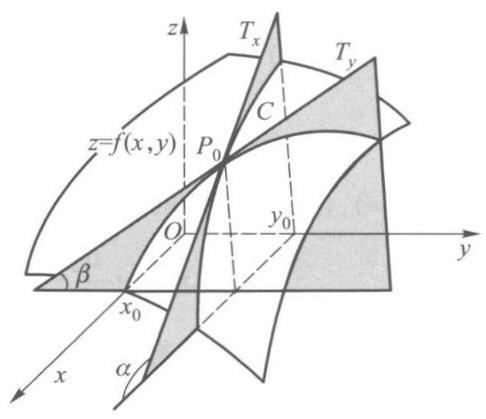
\includegraphics[width=.3\textwidth]{images/P128.jpg}
	\caption{图 $17-1$}
	\label{fig:P128}
\end{figure}

在点 \({P}_{0}\) 处的切线 \({T}_{y}\) 关于 \(y\) 轴的斜率 \(\tan \beta\) .

由偏导数的定义还知道,函数 \(f\) 对某一个自变量求偏导数, 是先把其他自变量看作常数, 从而变成一元函数的求导问题. 因此第五章中有关求导的一些基本法则, 对多元函数求偏导数仍然适用.

%例 2
\begin{example}

\end{example}
求函数 \(f\left( {x,y}\right)  = {x}^{3} + 2{x}^{2}y - {y}^{3}\) 在点(1,3)关于 \(x\) 和关于 \(y\) 的偏导数.

%解
\begin{solution}

\end{solution}
先求 \(f\) 在点(1,3)关于 \(x\) 的偏导数,为此,令 \(y = 3\) ,得到以 \(x\) 为自变量的函数 \(f\left( {x,3}\right)  = {x}^{3} + 6{x}^{2} - {27}\) ,求它在 \(x = 1\) 的导数,即
\[
{f}_{x}\left( {1,3}\right)  = {\left. \frac{\mathrm{d}f\left( {x,3}\right) }{\mathrm{d}x}\right| }_{x = 1} = 3{x}^{2} + {\left. {12}x\right| }_{x = 1} = {15}.
\]
再求 \(f\) 在(1,3)关于 \(y\) 的偏导数. 先令 \(x = 1\) ,得到以 \(y\) 为自变量的函数 \(f\left( {1,y}\right)  = 1 +\)  \({2y} - {y}^{3}\) ,求它在 \(y = 3\) 的导数,得
\[
{f}_{y}\left( {1,3}\right)  = {\left. \frac{\mathrm{d}f\left( {1,y}\right) }{\mathrm{d}y}\right| }_{y = 3} = {\left. 2 - 3{y}^{2}\right| }_{y = 3} =  - {25}.
\]
通常也可分别先求出 \(f\) 关于 \(x\) 和 \(y\) 的偏导函数:
\[
{f}_{x}\left( {x,y}\right)  = 3{x}^{2} + {4xy},
\]
\[
{f}_{y}\left( {x,y}\right)  = 2{x}^{2} - 3{y}^{2}.
\]
然后以 \(\left( {x,y}\right)  = \left( {1,3}\right)\) 代入,也能得到同样结果.

%例 3
\begin{example}

\end{example}
求函数 \(z = {x}^{y}\left( {x > 0}\right)\) 的偏导数.

解
\[
\frac{\partial z}{\partial x} = y{x}^{y - 1},\;\frac{\partial z}{\partial y} = {x}^{y}\ln x.
\]
%例 4
\begin{example}

\end{example}
求三元函数 \(u = \sin \left( {x + {y}^{2} - {\mathrm{e}}^{z}}\right)\) 的偏导数.

%解
\begin{solution}

\end{solution}
把 \(y\) 和 \(z\) 看作常数,得
\[
\frac{\partial u}{\partial x} = \cos \left( {x + {y}^{2} - {\mathrm{e}}^{z}}\right) .
\]
把 \(x,z\) 看作常数,得
\[
\frac{\partial u}{\partial y} = {2y}\cos \left( {x + {y}^{2} - {\mathrm{e}}^{z}}\right) .
\]
把 \(x,y\) 看作常数,得
\[
\frac{\partial u}{\partial z} =  - {\mathrm{e}}^{z}\cos \left( {x + {y}^{2} - {\mathrm{e}}^{z}}\right) .
\]
\subsection{可微性条件}

由偏导数定义及 (5), (6) 两式可得如下定理.

%定理 17.1
\begin{theorem}{}{the:}

\end{theorem}
 (可微的必要条件) 若二元函数 \(f\) 在其定义域内一点 \(\left( {{x}_{0},{y}_{0}}\right)\) 可微,则 \(f\) 在该点关于每个自变量的偏导数都存在,且 (1) 式中的
\[
A = {f}_{x}\left( {{x}_{0},{y}_{0}}\right) ,\;B = {f}_{y}\left( {{x}_{0},{y}_{0}}\right) .
\]
因此,函数 \(f\) 在点 \(\left( {{x}_{0},{y}_{0}}\right)\) 的全微分 (2) 可惟一地表示为
\[
{\left. \mathrm{d}f\right| }_{\left( {x}_{0},{y}_{0}\right) } = {f}_{x}\left( {{x}_{0},{y}_{0}}\right)  \cdot  {\Delta x} + {f}_{y}\left( {{x}_{0},{y}_{0}}\right)  \cdot  {\Delta y}.
\]
与一元函数的情况一样, 由于自变量的增量等于自变量的微分, 即
\[
{\Delta x} = \mathrm{d}x,\;{\Delta y} = \mathrm{d}y,
\]
所以 \(f\) 在点 \(\left( {{x}_{0},{y}_{0}}\right)\) 的全微分又可写为
\[
\mathrm{d}z = {f}_{x}\left( {{x}_{0},{y}_{0}}\right) \mathrm{d}x + {f}_{y}\left( {{x}_{0},{y}_{0}}\right) \mathrm{d}y.
\]
若函数 \(f\) 在区域 \(D\) 上每一点(x, y)都可微,则称函数 \(f\) 在区域 \(D\) 上可微,且 \(f\) 在 \(D\) 上全微分为
\[
\mathrm{d}f\left( {x,y}\right)  = {f}_{x}\left( {x,y}\right) \mathrm{d}x + {f}_{y}\left( {x,y}\right) \mathrm{d}y. \tag{8}
\]
%例 5
\begin{example}

\end{example}
考察函数
\[
f\left( {x,y}\right)  = \left\{  \begin{array}{ll} \frac{xy}{\sqrt{{x}^{2} + {y}^{2}}}, & {x}^{2} + {y}^{2} \neq  0, \\  0, & {x}^{2} + {y}^{2} = 0 \end{array}\right.
\]
在原点的可微性.

%解
\begin{solution}

\end{solution}
按偏导数定义
\[
{f}_{x}\left( {0,0}\right)  = \mathop{\lim }\limits_{{{\Delta x} \rightarrow  0}}\frac{f\left( {{\Delta x},0}\right)  - f\left( {0,0}\right) }{\Delta x} = \mathop{\lim }\limits_{{{\Delta x} \rightarrow  0}}\frac{0 - 0}{\Delta x} = 0.
\]
同理可得 \({f}_{y}\left( {0,0}\right)  = 0\) . 若函数 \(f\) 在原点可微,则
\[
{\Delta z} - \mathrm{d}z = f\left( {0 + {\Delta x},0 + {\Delta y}}\right)  - f\left( {0,0}\right)  - {f}_{x}\left( {0,0}\right) {\Delta x} - {f}_{y}\left( {0,0}\right) {\Delta y}
\]
\[
= \frac{\Delta x\Delta y}{\sqrt{\Delta {x}^{2} + \Delta {y}^{2}}}
\]
应是较 \(\rho  = \sqrt{\Delta {x}^{2} + \Delta {y}^{2}}\) 高阶的无穷小量. 为此,考察极限
\[
\mathop{\lim }\limits_{{\rho  \rightarrow  0}}\frac{{\Delta z} - \mathrm{d}z}{\rho } = \mathop{\lim }\limits_{{\rho  \rightarrow  0}}\frac{\Delta x\Delta y}{\Delta {x}^{2} + \Delta {y}^{2}},
\]
由第十六章 §2 例 3 知道,上述极限不存在,因而函数 \(f\) 在原点不可微.

我们知道, 一元函数可微与存在导数是等价的. 而例 5 说明对于多元函数, 偏导数即使都存在, 该函数也不一定可微. 现在不禁要问: 当所有偏导数都存在时, 还需要添加哪些条件, 才能保证函数可微呢?

%定理 17.2
\begin{theorem}{}{the:}

\end{theorem}
 (可微的充分条件) 若函数 \(z = f\left( {x,y}\right)\) 的偏导数在点 \(\left( {{x}_{0},{y}_{0}}\right)\) 的某邻域内存在,且 \({f}_{x}\) 与 \({f}_{y}\) 在点 \(\left( {{x}_{0},{y}_{0}}\right)\) 连续,则函数 \(f\) 在点 \(\left( {{x}_{0},{y}_{0}}\right)\) 可微.

%证
\begin{proof}

\end{proof}
我们把全增量 \({\Delta z}\) 写作
\[
{\Delta z} = f\left( {{x}_{0} + {\Delta x},{y}_{0} + {\Delta y}}\right)  - f\left( {{x}_{0},{y}_{0}}\right)
\]
\[
= \left\lbrack  {f\left( {{x}_{0} + {\Delta x},{y}_{0} + {\Delta y}}\right)  - f\left( {{x}_{0},{y}_{0} + {\Delta y}}\right) }\right\rbrack   + \left\lbrack  {f\left( {{x}_{0},{y}_{0} + {\Delta y}}\right)  - f\left( {{x}_{0},{y}_{0}}\right) }\right\rbrack  .
\]
在第一个括号里,它是函数 \(f\left( {x,{y}_{0} + {\Delta y}}\right)\) 关于 \(x\) 的偏增量. 在第二个括号里,则是函数 \(f\left( {{x}_{0},y}\right)\) 关于 \(y\) 的偏增量. 对它们分别应用一元函数的拉格朗日中值定理,得
\[
{\Delta z} = {f}_{x}\left( {{x}_{0} + {\theta }_{1}{\Delta x},{y}_{0} + {\Delta y}}\right) {\Delta x} + {f}_{y}\left( {{x}_{0},{y}_{0} + {\theta }_{2}{\Delta y}}\right) {\Delta y},0 < {\theta }_{1},{\theta }_{2} < 1. \tag{9}
\]
由于 \({f}_{x}\) 与 \({f}_{y}\) 在点 \(\left( {{x}_{0},{y}_{0}}\right)\) 连续,因此有
\[
{f}_{x}\left( {{x}_{0} + {\theta }_{1}{\Delta x},{y}_{0} + {\Delta y}}\right)  = {f}_{x}\left( {{x}_{0},{y}_{0}}\right)  + \alpha , \tag{10}
\]
\[
{f}_{y}\left( {{x}_{0},{y}_{0} + {\theta }_{2}{\Delta y}}\right)  = {f}_{y}\left( {{x}_{0},{y}_{0}}\right)  + \beta , \tag{11}
\]
其中当 \(\left( {{\Delta x},{\Delta y}}\right)  \rightarrow  \left( {0,0}\right)\) 时, \(\alpha  \rightarrow  0,\beta  \rightarrow  0\) . 将 (10) 式、(11) 式代入 (9) 式,则得
\[
{\Delta z} = {f}_{x}\left( {{x}_{0},{y}_{0}}\right) {\Delta x} + {f}_{y}\left( {{x}_{0},{y}_{0}}\right) {\Delta y} + {\alpha \Delta x} + {\beta \Delta y}.
\]
由 (4) 式便知函数 \(f\) 在点 \(\left( {{x}_{0},{y}_{0}}\right)\) 可微.

根据这个定理,例 2 中的函数 \(f\left( {x,y}\right)  = {x}^{3} + 2{x}^{2}y - {y}^{3}\) 在点(1,3)可微,且
\[
{\left. \mathrm{d}f\right| }_{\left( 1,3\right) } = {15}\mathrm{\;d}x - {25}\mathrm{\;d}y.
\]
%例 3
\begin{example}

\end{example}
中的函数 \(z = {x}^{y}\) 在 \(D = \{ \left( {x,y}\right)  \mid  x > 0, - \infty  < y <  + \infty \}\) 上可微,且
\[
\mathrm{d}z = y{x}^{y - 1}\mathrm{\;d}x + {x}^{y}\ln x\mathrm{\;d}y.
\]
%注
\begin{remark}

\end{remark}
偏导数连续并不是函数可微的必要条件, 如函数
\[
f\left( {x,y}\right)  = \left\{  \begin{matrix} \left( {{x}^{2} + {y}^{2}}\right) \sin \frac{1}{\sqrt{{x}^{2} + {y}^{2}}}, & {x}^{2} + {y}^{2} \neq  0, \\  0, & {x}^{2} + {y}^{2} = 0 \end{matrix}\right.
\]
在原点(0,0)可微,但 \({f}_{x}\) 与 \({f}_{y}\) 却在点(0,0)不连续 (见本节习题 7). 若 \(z = f\left( {x,y}\right)\) 在点 \(\left( {{x}_{0},{y}_{0}}\right)\) 的偏导数 \({f}_{x},{f}_{y}\) 连续,则称 \(f\) 在点 \(\left( {{x}_{0},{y}_{0}}\right)\) 连续可微.

在定理 17.2 证明过程中所出现的 (9) 式, 实际上是二元函数的一个中值公式, 可以将其归纳为下述定理.

%定理 17.3
\begin{theorem}{}{the:}

\end{theorem}
 设函数 \(f\) 在点 \(\left( {{x}_{0},{y}_{0}}\right)\) 的某邻域内存在偏导数,若(x, y)属于该邻域, 则存在 \(\xi  = {x}_{0} + {\theta }_{1}\left( {x - {x}_{0}}\right)\) 和 \(\eta  = {y}_{0} + {\theta }_{2}\left( {y - {y}_{0}}\right) ,0 < {\theta }_{1},{\theta }_{2} < 1\) ,使得
\[
f\left( {x,y}\right)  - f\left( {{x}_{0},{y}_{0}}\right)  = {f}_{x}\left( {\xi ,y}\right) \left( {x - {x}_{0}}\right)  + {f}_{y}\left( {{x}_{0},\eta }\right) \left( {y - {y}_{0}}\right) . \tag{12}
\]
读者还可以从可微性概念看到, 函数在可微点处必连续, 但在函数的连续点处不一定存在偏导数,当然它更不能保证函数在该点可微. 例如,函数 \(f\left( {x,y}\right)  = \sqrt{{x}^{2} + {y}^{2}}\) (圆锥) 在原点连续, 但在该点不存在偏导数. 更值得注意的是, 即使函数在某一点存在对所有自变量的偏导数, 也不能保证函数在该点连续. 例如,
\[
f\left( {x,y}\right)  = \left\{  \begin{matrix} \frac{xy}{{x}^{2} + {y}^{2}}, & {x}^{2} + {y}^{2} \neq  0, \\  0, & {x}^{2} + {y}^{2} = 0 \end{matrix}\right.
\]
在原点不连续, 但却存在偏导数
\[
{f}_{x}\left( {0,0}\right)  = \mathop{\lim }\limits_{{{\Delta x} \rightarrow  0}}\frac{0 - 0}{\Delta x} = 0,\;{f}_{y}\left( {0,0}\right)  = 0.
\]
这是因为偏导数只是刻画了函数沿 \(x\) 轴或 \(y\) 轴方向的变化特征,所以这个例子只能说明 \(f\) 在原点分别对 \(x\) 和对 \(y\) 必定连续,但由此并不能保证 \(f\) 作为二元函数在原点连续. 与定理 17.2 相仿, 只有对偏导数附加适当的条件后, 才能保证函数的连续性 (有关内容可从本节习题中去找).

\subsection{可微性几何意义及应用}

一元函数可微,在几何上反映为曲线存在不平行于 \(y\) 轴的切线. 对于二元函数来说, 可微性则反映为曲面与其切平面之间的类似关系. 为此, 我们需要先给出曲面的切平面的定义, 这可以从曲线的切线定义中获得启发.

在第五章 §1 中,我们曾把平面曲线 \(S\) 在某一点 \(P\left( {{x}_{0},{y}_{0}}\right)\) 的切线 \({PT}\) 定义为过 \(P\) 点的割线 \({PQ}\) 当 \(Q\) 沿 \(S\) 趋近 \(P\) 时的极限位置 (如果存在的话). 这时, \({PQ}\) 与 \({PT}\) 的夹角 \(\varphi\) 也将随 \(Q \rightarrow  P\) 而趋于零 (图 17-2). 由于
\[
\sin \varphi  = \frac{h}{d},
\]
其中 \(h\) 和 \(d\) 分别表示点 \(Q\) 到切线 \({PT}\) 的距离和 \(Q\) 到 \(P\) 的距离,因此当 \(Q\) 沿 \(S\) 趋于 \(P\) 时, \(\varphi  \rightarrow  0\) 等同于 \(\frac{h}{d} \rightarrow  0\) .

仿照这个想法,我们引入曲面 \(S\) 在点 \(P\) 的切平面定义.

%定义  3
\begin{definition}{}{def:}

\end{definition}
设 \(P\) 是曲面 \(S\) 上一点, \(\Pi\) 为通过点 \(P\) 的一个平面,曲面 \(S\) 上的动点 \(Q\) 到定点 \(P\) 和到平面 \(\Pi\) 的距离分别为 \(d\) 与 \(h\) (图 17-3). 若当 \(Q\) 在 \(S\) 上以任何方式趋近于 \(P\) 时,恒有 \(\frac{h}{d} \rightarrow  0\) ,则称平面 \(\Pi\) 为曲面 \(S\) 在点 \(P\) 处的切平面, \(P\) 为切点.

\begin{figure}
	\centering
	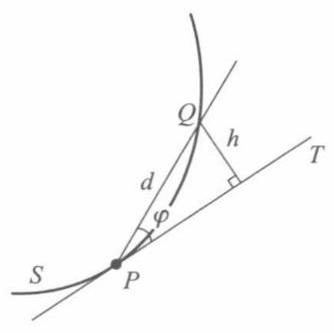
\includegraphics[width=.3\textwidth]{images/P129.jpg}
	\caption{图 $17-2$}
	\label{fig:P129}
\end{figure}

\begin{figure}
	\centering
	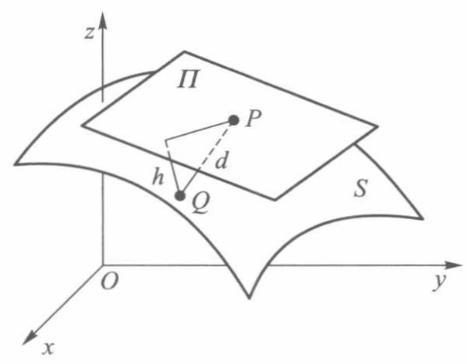
\includegraphics[width=.3\textwidth]{images/P130.jpg}
	\caption{图 $17-3$}
	\label{fig:P130}
\end{figure}

%定理 17.4
\begin{theorem}{}{the:}

\end{theorem}
 曲面 \(z = f\left( {x,y}\right)\) 在点 \(P\left( {{x}_{0},{y}_{0},f\left( {{x}_{0},{y}_{0}}\right) }\right)\) 存在不平行于 \(z\) 轴的切平面 \(\Pi\) 的充要条件是函数 \(f\) 在点 \({P}_{0}\left( {{x}_{0},{y}_{0}}\right)\) 可微.

%证
\begin{proof}

\end{proof}
[充分性] 若函数 \(f\) 在 \({P}_{0}\) 处可微,由定义知
\[
{\Delta z} = z - {z}_{0} = {f}_{x}\left( {{x}_{0},{y}_{0}}\right) \left( {x - {x}_{0}}\right)  + {f}_{y}\left( {{x}_{0},{y}_{0}}\right) \left( {y - {y}_{0}}\right)  + o\left( \rho \right) ,
\]
其中 \({z}_{0} = f\left( {{x}_{0},{y}_{0}}\right) ,\rho  = \sqrt{{\left( x - {x}_{0}\right) }^{2} + {\left( y - {y}_{0}\right) }^{2}}\) . 现在讨论过点 \(P\left( {{x}_{0},{y}_{0},{z}_{0}}\right)\) 的平面
\[
Z - {z}_{0} = {f}_{x}\left( {{x}_{0},{y}_{0}}\right) \left( {X - {x}_{0}}\right)  + {f}_{y}\left( {{x}_{0},{y}_{0}}\right) \left( {Y - {y}_{0}}\right) ,
\]
其中 \(X,Y,Z\) 是平面上任意点的坐标. 我们证明它就是曲面 \(z = f\left( {x,y}\right)\) 在点 \(P\) 的切平面 \(\Pi\) . 事实上,由解析几何学知道,曲面上任意一点 \(Q\left( {x,y,z}\right)\) 到这个平面的距离为
\[
h = \frac{\left| z - {z}_{0} - {f}_{x}\left( {x}_{0},{y}_{0}\right) \left( x - {x}_{0}\right)  - {f}_{y}\left( {x}_{0},{y}_{0}\right) \left( y - {y}_{0}\right) \right| }{\sqrt{1 + {f}_{x}^{2}\left( {{x}_{0},{y}_{0}}\right)  + {f}_{y}^{2}\left( {{x}_{0},{y}_{0}}\right) }}
\]
\[
= \frac{\left| o\left( \rho \right) \right| }{\sqrt{1 + {f}_{x}^{2}\left( {{x}_{0},{y}_{0}}\right)  + {f}_{y}^{2}\left( {{x}_{0},{y}_{0}}\right) }},
\]
另一方面, \(P\) 到 \(Q\) 的距离为
\[
d = \sqrt{{\left( x - {x}_{0}\right) }^{2} + {\left( y - {y}_{0}\right) }^{2} + {\left( z - {z}_{0}\right) }^{2}} = \sqrt{{\rho }^{2} + {\left( z - {z}_{0}\right) }^{2}} \geq  \rho .
\]
于是由 \(\frac{h}{d} \geq  0\) 及
\[
\frac{h}{d} < \frac{h}{\rho } = \frac{\left| o\left( \rho \right) \right| }{\rho }\frac{1}{\sqrt{1 + {f}_{x}^{2}\left( {{x}_{0},{y}_{0}}\right)  + {f}_{y}^{2}\left( {{x}_{0},{y}_{0}}\right) }} \rightarrow  0\left( {\rho  \rightarrow  0}\right) ,
\]
根据定义 3,平面 \(\Pi\) 为曲面 \(z = f\left( {x,y}\right)\) 在点 \(P\) 的切平面.

[必要性] 若曲面 \(z = f\left( {x,y}\right)\) 在点 \(P\left( {{x}_{0},{y}_{0},f\left( {{x}_{0},{y}_{0}}\right) }\right)\) 存在不平行于 \(z\) 轴的切平面
\[
Z - {z}_{0} = A\left( {X - {x}_{0}}\right)  + B\left( {Y - {y}_{0}}\right) ,
\]
且 \(Q\left( {x,y,z}\right)\) 是曲面上任意一点,则点 \(Q\) 到这个平面的距离为
\[
h = \frac{\left| z - {z}_{0} - A\left( x - {x}_{0}\right)  - B\left( y - {y}_{0}\right) \right| }{\sqrt{1 + {A}^{2} + {B}^{2}}}.
\]
令 \(x - {x}_{0} = {\Delta x},y - {y}_{0} = {\Delta y},z - {z}_{0} = {\Delta z},\rho  = \sqrt{\Delta {x}^{2} + \Delta {y}^{2}}\) . 由切平面定义知,当 \(Q\) 充分接近 \(P\) 时,有 \(\frac{h}{d} \rightarrow  0\) .

要证明 \(f\) 在 \({P}_{0}\left( {{x}_{0},{y}_{0}}\right)\) 可微,就是要证明
\[
\mathop{\lim }\limits_{{\rho  \rightarrow  0}}\frac{\left| \Delta z - A\Delta x - B\Delta y\right| }{\rho } = 0.
\]
由于
\[
\frac{\left| \Delta z - A\Delta x - B\Delta y\right| }{\rho } = \frac{\left| \Delta z - A\Delta x - B\Delta y\right| }{d\sqrt{1 + {A}^{2} + {B}^{2}}} \cdot  \frac{d}{\rho } \cdot  \sqrt{1 + {A}^{2} + {B}^{2}}
\]
\[
= \frac{h}{d} \cdot  \frac{d}{\rho } \cdot  \sqrt{1 + {A}^{2} + {B}^{2}},
\]
而 \(\frac{h}{d} \rightarrow  0\left( {\rho  \rightarrow  0}\right)\) ,故只需证明当 \(\rho\) 充分小时, \(\frac{d}{\rho }\) 有界即可.

对于充分接近 \(P\) 的 \(Q\) ,有
\[
0 < \frac{h}{d} = \frac{\left| \Delta z - A\Delta x - B\Delta y\right| }{d\sqrt{1 + {A}^{2} + {B}^{2}}} < \frac{1}{2\sqrt{1 + {A}^{2} + {B}^{2}}},
\]
由此得
\[
\left| {{\Delta z} - {A\Delta x} - {B\Delta y}}\right|  < \frac{d}{2} = \frac{1}{2}\sqrt{\Delta {x}^{2} + \Delta {y}^{2} + \Delta {z}^{2}} = \frac{1}{2}\sqrt{{\rho }^{2} + \Delta {z}^{2}}.
\]
由 \(\left| a\right|  - \left| b\right|  \leq  \left| {a - b}\right|\) ,可得
\[
\left| {\Delta z}\right|  - \left| A\right| \left| {\Delta x}\right|  - \left| B\right| \left| {\Delta y}\right|  < \frac{1}{2}\sqrt{{\rho }^{2} + \Delta {z}^{2}} \leq  \frac{1}{2}\left( {\rho  + \left| {\Delta z}\right| }\right) ,
\]
故有
\[
\frac{1}{2}\left| {\Delta z}\right|  < \left| A\right| \left| {\Delta x}\right|  + \left| B\right| \left| {\Delta y}\right|  + \frac{1}{2}\rho ,
\]
\[
\frac{\left| \Delta z\right| }{\rho } < 2\left( {\left| A\right| \frac{\left| \Delta x\right| }{\rho } + \left| B\right| \frac{\left| \Delta y\right| }{\rho }}\right)  + 1 \leq  2\left( {\left| A\right|  + \left| B\right| }\right)  + 1.
\]
因此 \(\frac{\left| \Delta z\right| }{\rho }\) 是有界量. 从而推得 \(\frac{d}{\rho } = \frac{\sqrt{{\rho }^{2} + \Delta {z}^{2}}}{\rho } = \sqrt{1 + {\left( \frac{\Delta z}{\rho }\right) }^{2}}\) 也是有界量.

根据前面的分析, 有
\[
\mathop{\lim }\limits_{{\rho  \rightarrow  0}}\frac{\left| \Delta z - A\Delta x - B\Delta y\right| }{\rho } = 0.
\]
即
\[
{\Delta z} = {A\Delta x} + {B\Delta y} + o\left( \rho \right) .
\]
这就证明了函数 \(z = f\left( {x,y}\right)\) 在点 \({P}_{0}\left( {{x}_{0},{y}_{0}}\right)\) 是可微的.

%定理 17.4
\begin{theorem}{}{the:}

\end{theorem}
 说明: 若函数 \(f\) 在点 \({P}_{0}\left( {{x}_{0},{y}_{0}}\right)\) 可微,则曲面 \(z = f\left( {x,y}\right)\) 在点 \(P\left( {{x}_{0},{y}_{0},{z}_{0}}\right)\) 的切平面方程为
\[
z - {z}_{0} = {f}_{x}\left( {{x}_{0},{y}_{0}}\right) \left( {x - {x}_{0}}\right)  + {f}_{y}\left( {{x}_{0},{y}_{0}}\right) \left( {y - {y}_{0}}\right) . \tag{13}
\]
过切点 \(P\) 与切平面垂直的直线称为曲面在点 \(P\) 的法线. 由切平面方程知道,法线的方向数是
\[
\pm  \left( {{f}_{x}\left( {{x}_{0},{y}_{0}}\right) ,{f}_{y}\left( {{x}_{0},{y}_{0}}\right) , - 1}\right) ,
\]
所以过切点 \(P\) 的法线方程是
\[
\frac{x - {x}_{0}}{{f}_{x}\left( {{x}_{0},{y}_{0}}\right) } = \frac{y - {y}_{0}}{{f}_{y}\left( {{x}_{0},{y}_{0}}\right) } = \frac{z - {z}_{0}}{-1}. \tag{14}
\]
二元函数全微分的几何意义如图 17-4 所示,当自变量 \(x,y\) 的增量分别为 \({\Delta x},{\Delta y}\) 时,函数 \(z = f\left( {x,y}\right)\) 的增量 \({\Delta z}\) 是竖坐标上的一段 \({NQ}\) , 而二元函数 \(z = f\left( {x,y}\right)\) 在点 \(\left( {{x}_{0},{y}_{0}}\right)\) 的全微分
\[
\mathrm{d}z = {f}_{x}\left( {{x}_{0},{y}_{0}}\right) {\Delta x} + {f}_{y}\left( {{x}_{0},{y}_{0}}\right) {\Delta y}
\]
\begin{figure}
	\centering
	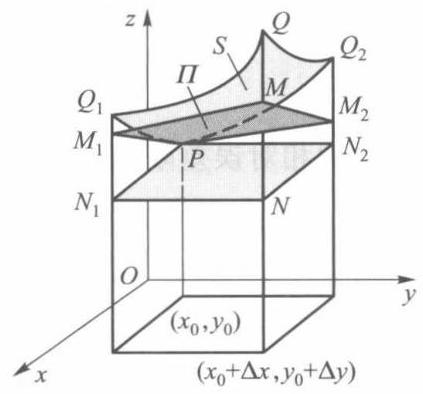
\includegraphics[width=.3\textwidth]{images/P131.jpg}
	\caption{图 $17-4$}
	\label{fig:P131}
\end{figure}

的值是过点 \(P\) 的切平面 \(P{M}_{1}M{M}_{2}\) 上相应的增量 \({NM}\) . 于是 \({\Delta z}\) 与 \(\mathrm{d}z\) 之差是 \({MQ}\) ,它的值随着 \(\rho  \rightarrow  0\) 而趋于零, 而且是较 \(\rho\) 高阶的无穷小量.

%例 6
\begin{example}

\end{example}
试求抛物面 \(z = a{x}^{2} + b{y}^{2}\) 在曲面上一点 \(M\left( {{x}_{0},{y}_{0},{z}_{0}}\right)\) 处的切平面方程与法线方程. 解 因为
\[
{f}_{x}\left( {{x}_{0},{y}_{0}}\right)  = {2a}{x}_{0},\;{f}_{y}\left( {{x}_{0},{y}_{0}}\right)  = {2b}{y}_{0},
\]
由公式 (13),过 \(M\) 的切平面方程为
\[
z - {z}_{0} = {2a}{x}_{0}\left( {x - {x}_{0}}\right)  + {2b}{y}_{0}\left( {y - {y}_{0}}\right) .
\]
因为 \({z}_{0} = a{x}_{0}^{2} + b{y}_{0}^{2}\) ,所以它可简化为
\[
{2a}{x}_{0}x + {2b}{y}_{0}y - z - {z}_{0} = 0.
\]
由公式 (14),过点 \(M\) 的法线方程是
\[
\frac{x - {x}_{0}}{{2a}{x}_{0}} = \frac{y - {y}_{0}}{{2b}{y}_{0}} = \frac{z - {z}_{0}}{-1}.
\]
下面的例 7 和例 8 是利用线性近似公式 (3) 所作的近似计算和误差估计.

%例 7
\begin{example}

\end{example}
求 \({1.08}^{3.96}\) 的近似值.

%解
\begin{solution}

\end{solution}
设 \(f\left( {x,y}\right)  = {x}^{y}\) ,令 \({x}_{0} = 1,{y}_{0} = 4,{\Delta x} = {0.08},{\Delta y} =  - {0.04}\) . 由公式 (3) 有
\[
{1.08}^{3.96} = f\left( {{x}_{0} + {\Delta x},{y}_{0} + {\Delta y}}\right)
\]
\[
\approx  f\left( {1,4}\right)  + {f}_{x}\left( {1,4}\right) {\Delta x} + {f}_{y}\left( {1,4}\right) {\Delta y}
\]
\[
= 1 + 4 \times  {0.08} + {1}^{4} \times  \ln 1 \times  \left( {-{0.04}}\right)
\]
\[
= 1 + {0.32} = {1.32}\text{ . }
\]
%例 8
\begin{example}

\end{example}
应用公式 \(S = \frac{1}{2}{ab}\sin C\) 计算某三角形面积,现测得 \(a = {12.50},b = {8.30},C =\)  \({30}^{ \circ  }\) . 若测量 \(a,b\) 的误差为 \(\pm  {0.01},C\) 的误差为 \(\pm  {0.1}^{ \circ  }\) ,求用此公式计算三角形面积时的绝对误差限与相对误差限.

%解
\begin{solution}

\end{solution}
依题意,测量中 \(a,b,C\) 的绝对误差限分别为
\[
\left| {\Delta a}\right|  = {0.01},\;\left| {\Delta b}\right|  = {0.01},\;\left| {\Delta C}\right|  = {0.1}^{ \circ  } = \frac{\pi }{1800}.
\]
由于
\[
\left| {\Delta S}\right|  \approx  \left| {\mathrm{d}S}\right|  = \left| {\frac{\partial S}{\partial a}{\Delta a} + \frac{\partial S}{\partial b}{\Delta b} + \frac{\partial S}{\partial C}{\Delta C}}\right|
\]
\[
\leq  \left| \frac{\partial S}{\partial a}\right| \left| {\Delta a}\right|  + \left| \frac{\partial S}{\partial b}\right| \left| {\Delta b}\right|  + \left| \frac{\partial S}{\partial C}\right| \left| {\Delta C}\right|
\]
\[
= \frac{1}{2}\left| {b\sin C}\right| \left| {\Delta a}\right|  + \frac{1}{2}\left| {a\sin C}\right| \left| {\Delta b}\right|  + \frac{1}{2}\left| {{ab}\cos C}\right| \left| {\Delta C}\right| \text{ , }
\]
将各数据代入上式,得到 \(S\) 的绝对误差限为
\[
\left| {\Delta S}\right|  \approx  {0.13}\text{ . }
\]
因为
\[
S = \frac{1}{2}{ab}\sin C = \frac{1}{2} \times  {12.50} \times  {8.30} \times  \frac{1}{2} \approx  {25.94},
\]
所以 \(S\) 的相对误差限为
\[
\left| \frac{\Delta S}{S}\right|  \approx  \frac{0.13}{25.94} \approx  {0.5}\% .
\]
\subsection{习题 17.1}

1. 求下列函数的偏导数:

(1) \(z = {x}^{2}y\) ;

(2) \(z = y\cos x\) ;

(3) \(z = \frac{1}{\sqrt{{x}^{2} + {y}^{2}}}\) ;

(4) \(z = \ln \left( {x + {y}^{2}}\right)\) ;

(5) \(z = {\mathrm{e}}^{xy}\) ;

(6) \(z = \arctan \frac{y}{x}\) ;

(7) \(z = {xy}{\mathrm{e}}^{\sin \left( {xy}\right) }\) ;

(8) \(u = \frac{y}{x} + \frac{z}{y} - \frac{x}{z}\) ;

(9) \(u = {\left( xy\right) }^{2}\) ;

(10) \(u = {x}^{{y}^{z}}\) .

2. 设 \(f\left( {x,y}\right)  = x + \left( {y - 1}\right) \arcsin \sqrt{\frac{x}{y}}\) ,求 \({f}_{x}\left( {x,1}\right)\) .

3. 设 \(f\left( {x,y}\right)  = \left\{  \begin{matrix} y\sin \frac{1}{{x}^{2} + {y}^{2}}, & {x}^{2} + {y}^{2} \neq  0, \\  0, & {x}^{2} + {y}^{2} = 0, \end{matrix}\right.\) 考察函数 \(f\) 在原点(0,0)的偏导数.

4. 证明函数 \(z = \sqrt{{x}^{2} + {y}^{2}}\) 在点(0,0)连续但偏导数不存在.

5. 考察函数 \(f\left( {x,y}\right)  = \left\{  \begin{matrix} {xy}\sin \frac{1}{{x}^{2} + {y}^{2}}, & {x}^{2} + {y}^{2} \neq  0, \\  0, & {x}^{2} + {y}^{2} = 0 \end{matrix}\right.\) 在点(0,0)的可微性.

6. 证明函数 \(f\left( {x,y}\right)  = \left\{  \begin{matrix} \frac{{x}^{2}y}{{x}^{2} + {y}^{2}}, & {x}^{2} + {y}^{2} \neq  0, \\  0, & {x}^{2} + {y}^{2} = 0 \end{matrix}\right.\) 在点(0,0)连续且偏导数存在,但在此点不可微.

7. 证明函数 \(f\left( {x,y}\right)  = \left\{  \begin{matrix} \left( {{x}^{2} + {y}^{2}}\right) \sin \frac{1}{\sqrt{{x}^{2} + {y}^{2}}}, & {x}^{2} + {y}^{2} \neq  0, \\  0, & {x}^{2} + {y}^{2} = 0 \end{matrix}\right.\) 在点(0,0)连续且偏导数存在,但偏导数在点(0,0)不连续,而 \(f\) 在点(0,0)可微.

8. 求下列函数在给定点的全微分:

(1) \(z = {x}^{4} + {y}^{4} - 4{x}^{2}{y}^{2}\) 在点 \(\left( {0,0}\right) ,\left( {1,1}\right)\) ;

(2) \(z = \frac{x}{\sqrt{{x}^{2} + {y}^{2}}}\) 在点 \(\left( {1,0}\right) ,\left( {0,1}\right)\) .

9. 求下列函数的全微分:

(1) \(z = y\sin \left( {x + y}\right)\) ;

(2) \(u = x{\mathrm{e}}^{yz} + {\mathrm{e}}^{-z} + y\) .

10. 求曲面 \(z = \arctan \frac{y}{x}\) 在点 \(\left( {1,1,\frac{\pi }{4}}\right)\) 的切平面方程和法线方程.

11. 求曲面 \(3{x}^{2} + {y}^{2} - {z}^{2} = {27}\) 在点(3,1,1)的切平面与法线方程.

12. 在曲面 \(z = {xy}\) 上求一点,使这点的切平面平行于平面 \(x + {3y} + z + 9 = 0\) ,并写出此切平面方程和法线方程.

13. 计算近似值:

(1) \({1.002} \times  {2.003}^{2} \times  {3.004}^{3}\) ;

(2) \(\sin {29}^{ \circ  } \times  \tan {46}^{ \circ  }\) .

14. 设圆台上、下底的半径分别为 \(R = {30}\mathrm{\;{cm}},r = {20}\mathrm{\;{cm}}\) ,高 \(h = {40}\mathrm{\;{cm}}\) . 若 \(R,r,h\) 分别增加 \(3\mathrm{\;{mm}}\) , \(4\mathrm{\;{mm}},2\mathrm{\;{mm}}\) ,求此圆台体积变化的近似值.

15. 证明: 若二元函数 \(f\) 在点 \(P\left( {{x}_{0},{y}_{0}}\right)\) 的某邻域 \(U\left( P\right)\) 上的偏导函数 \({f}_{x}\) 与 \({f}_{y}\) 有界,则 \(f\) 在 \(U\left( P\right)\) 上连续.

16. 设二元函数 \(f\) 在区域 \(D = \left\lbrack  {a,b}\right\rbrack   \times  \left\lbrack  {c,d}\right\rbrack\) 上连续.

(1) 若在 int \(D\) 内有 \({f}_{x} \equiv  0\) ,试问 \(f\) 在 \(D\) 上有何特性?

(2)若在 int \(D\) 内有 \({f}_{x} = {f}_{y} \equiv  0,f\) 又怎样？

(3)在(1)的讨论中,关于 \(f\) 在 \(D\) 上的连续性假设可否省略？长方形区域可否改为任意区域？

17. 试证在原点(0,0)的充分小邻域内,有
\[
\arctan \frac{x + y}{1 + {xy}} \approx  x + y.
\]
18. 求曲面 \(z = \frac{{x}^{2} + {y}^{2}}{4}\) 与平面 \(y = 4\) 的交线在 \(x = 2\) 处的切线与 \({Ox}\) 轴的交角.

19. 试证:(1)乘积的相对误差限近似于各因子相对误差限之和；

(2)商的相对误差限近似于分子和分母相对误差限之和.

20. 测得一物体的体积 \(V = {4.45}{\mathrm{\;{cm}}}^{3}\) ,其绝对误差限为 \({0.01}{\mathrm{\;{cm}}}^{3}\) ; 又测得质量 \(m = {30.80}\mathrm{\;g}\) ,其绝对误差限为 \({0.01}\mathrm{\;g}\) . 求由公式 \(\rho  = \frac{m}{V}\) 算出的密度 \(\rho\) 的相对误差限和绝对误差限.

\section{复合函数微分法}

本节讨论复合函数的可微性、偏导数与全微分.

\subsection{复合函数的求导法则}

设函数
\[
x = \varphi \left( {s,t}\right) \text{ 与 }y = \psi \left( {s,t}\right)  \tag{1}
\]
定义在 \({st}\) 平面的区域 \(D\) 上,函数
\[
z = f\left( {x,y}\right)  \tag{2}
\]
定义在 \({xy}\) 平面的区域 \({D}_{1}\) 上,且
\[
\{ \left( {x,y}\right)  \mid  x = \varphi \left( {s,t}\right) ,y = \psi \left( {s,t}\right) ,\left( {s,t}\right)  \in  D\}  \subset  {D}_{1},
\]
则函数
\[
z = F\left( {s,t}\right)  = f\left( {\varphi \left( {s,t}\right) ,\psi \left( {s,t}\right) }\right) ,\;\left( {s,t}\right)  \in  D \tag{3}
\]
是以 (2) 为外函数、(1) 为内函数的复合函数. 其中 \(x,y\) 称为函数 \(F\) 的中间变量, \(s,t\) 为 \(F\) 的自变量.

%定理 17.5
\begin{theorem}{}{the:}

\end{theorem}
 若函数 \(x = \varphi \left( {s,t}\right) ,y = \psi \left( {s,t}\right)\) 在点 \(\left( {s,t}\right)  \in  D\) 可微, \(z = f\left( {x,y}\right)\) 在点(x, y) \(= \left( {\varphi \left( {s,t}\right) ,\psi \left( {s,t}\right) }\right)\) 可微,则复合函数
\[
z = f\left( {\varphi \left( {s,t}\right) ,\psi \left( {s,t}\right) }\right)
\]
在点(s, t)可微,且它关于 \(s\) 与 \(t\) 的偏导数分别为
\[
{\left. \frac{\partial z}{\partial s}\right| }_{\left( s,t\right) } = {\left. {\left. \frac{\partial z}{\partial x}\right| }_{\left( x,y\right) }\frac{\partial x}{\partial s}\right| }_{\left( s,t\right) } + {\left. {\left. \frac{\partial z}{\partial y}\right| }_{\left( x,y\right) }\frac{\partial y}{\partial s}\right| }_{\left( s,t\right) }, \tag{4}
\]
\[
{\left. \frac{\partial z}{\partial t}\right| }_{\left( s,t\right) } = {\left. {\left. \frac{\partial z}{\partial x}\right| }_{\left( x,y\right) }\frac{\partial x}{\partial t}\right| }_{\left( s,t\right) } + {\left. {\left. \frac{\partial z}{\partial y}\right| }_{\left( x,y\right) }\frac{\partial y}{\partial t}\right| }_{\left( s,t\right) }.
\]
%证
\begin{proof}

\end{proof}
由假设 \(x = \varphi \left( {s,t}\right) ,y = \psi \left( {s,t}\right)\) 在点(s, t)可微,于是
\[
{\Delta x} = \frac{\partial x}{\partial s}{\Delta s} + \frac{\partial x}{\partial t}{\Delta t} + {\alpha }_{1}{\Delta s} + {\beta }_{1}{\Delta t}, \tag{5}
\]
\[
{\Delta y} = \frac{\partial y}{\partial s}{\Delta s} + \frac{\partial y}{\partial t}{\Delta t} + {\alpha }_{2}{\Delta s} + {\beta }_{2}{\Delta t}, \tag{6}
\]
其中当 \({\Delta s},{\Delta t}\) 趋于零时, \({\alpha }_{1},{\alpha }_{2},{\beta }_{1},{\beta }_{2}\) 都趋于零. 又由 \(z = f\left( {x,y}\right)\) 在点(x, y)可微,所以
\[
{\Delta z} = \frac{\partial z}{\partial x}{\Delta x} + \frac{\partial z}{\partial y}{\Delta y} + {\alpha \Delta x} + {\beta \Delta y}, \tag{7}
\]
其中当 \({\Delta x},{\Delta y} \rightarrow  0\) 时, \(\alpha ,\beta  \rightarrow  0\) (并补充定义当 \({\Delta x} = 0,{\Delta y} = 0\) 时 \(\alpha  = \beta  = 0\) ),将 (5) 式、(6) 式代入 (7) 式, 得
\[
{\Delta z} = \left( {\frac{\partial z}{\partial x} + \alpha }\right) \left( {\frac{\partial x}{\partial s}{\Delta s} + \frac{\partial x}{\partial t}{\Delta t} + {\alpha }_{1}{\Delta s} + {\beta }_{1}{\Delta t}}\right)  + \left( {\frac{\partial z}{\partial y} + \beta }\right) \left( {\frac{\partial y}{\partial s}{\Delta s} + \frac{\partial y}{\partial t}{\Delta t} + {\alpha }_{2}{\Delta s} + {\beta }_{2}{\Delta t}}\right) .
\]
整理后
\[
{\Delta z} = \left( {\frac{\partial z}{\partial x}\frac{\partial x}{\partial s} + \frac{\partial z}{\partial y}\frac{\partial y}{\partial s}}\right) {\Delta s} + \left( {\frac{\partial z}{\partial x}\frac{\partial x}{\partial t} + \frac{\partial z}{\partial y}\frac{\partial y}{\partial t}}\right) {\Delta t} + \bar{\alpha }{\Delta s} + \bar{\beta }{\Delta t}, \tag{8}
\]
其中
\[
\bar{\alpha } = \frac{\partial z}{\partial x}{\alpha }_{1} + \frac{\partial z}{\partial y}{\alpha }_{2} + \frac{\partial x}{\partial s}\alpha  + \frac{\partial y}{\partial s}\beta  + \alpha {\alpha }_{1} + \beta {\alpha }_{2}, \tag{9}
\]
\[
\bar{\beta } = \frac{\partial z}{\partial x}{\beta }_{1} + \frac{\partial z}{\partial y}{\beta }_{2} + \frac{\partial x}{\partial t}\alpha  + \frac{\partial y}{\partial t}\beta  + \alpha {\beta }_{1} + \beta {\beta }_{2}. \tag{10}
\]
由于 \(\varphi \left( {s,t}\right) ,\psi \left( {s,t}\right)\) 在点(s, t)可微,因此它们在点(s, t)都连续,即当 \({\Delta s},{\Delta t} \rightarrow  0\) 时,有 \({\Delta x},{\Delta y} \rightarrow  0\) . 从而也有 \(\alpha  \rightarrow  0,\beta  \rightarrow  0\) 以及 \({\alpha }_{1},{\alpha }_{2},{\beta }_{1},{\beta }_{2} \rightarrow  0\) . 于是在 (9) 式、(10) 式中,当 \({\Delta s}\) , \({\Delta t} \rightarrow  0\) 时,有 \(\bar{\alpha } \rightarrow  0,\bar{\beta } \rightarrow  0\) . 故由 (8) 式推得复合函数 (3) 可微并求得 \(z\) 关于 \(s\) 和 \(t\) 的偏导数 (4).

这里公式 (4) 也称为链式法则.

%注
\begin{remark}

\end{remark}
如果只是求复合函数 \(f\left( {\varphi \left( {s,t}\right) ,\psi \left( {s,t}\right) }\right)\) 关于 \(s\) 或 \(t\) 的偏导数,则定理 17.5 中 \(x = \varphi \left( {s,t}\right)\) 和 \(y = \psi \left( {s,t}\right)\) 只需具有关于 \(s\) 或 \(t\) 的偏导数就够了. 因为以 \({\Delta s}\) 或 \({\Delta t}\) 除 (7) 式两边,然后让 \({\Delta s} \rightarrow  0\) 或 \({\Delta t} \rightarrow  0\) ,也能得到相应的结果. 但是对外函数 \(f\) 的可微性假设是不能省略的, 否则上述复合函数求导公式不一定成立. 如函数
\[
f\left( {x,y}\right)  = \left\{  \begin{matrix} \frac{{x}^{2}y}{{x}^{2} + {y}^{2}}, & {x}^{2} + {y}^{2} \neq  0, \\  0, & {x}^{2} + {y}^{2} = 0. \end{matrix}\right.
\]
由 §1 习题 6 知 \({f}_{x}\left( {0,0}\right)  = {f}_{y}\left( {0,0}\right)  = 0\) ,但 \(f\left( {x,y}\right)\) 在(0,0)处不可微. 若以 \(f\left( {x,y}\right)\) 为外函数, \(x = t,y = t\) 为内函数,则得以 \(t\) 为自变量的复合函数
\[
z = F\left( t\right)  = f\left( {t,t}\right)  = \frac{t}{2},
\]
所以 \(\frac{\mathrm{d}z}{\mathrm{\;d}t} = \frac{1}{2}\) . 这时若用链式法则,将得出错误结果
\[
{\left. \frac{\mathrm{d}z}{\mathrm{\;d}t}\right| }_{t = 0} = {\left. {\left. \frac{\partial z}{\partial x}\right| }_{\left( 0,0\right) }\frac{\mathrm{d}x}{\mathrm{\;d}t}\right| }_{t = 0} + {\left. {\left. \frac{\partial z}{\partial y}\right| }_{\left( 0,0\right) }\frac{\mathrm{d}y}{\mathrm{\;d}t}\right| }_{t = 0}
\]
\[
= 0 \cdot  1 + 0 \cdot  1 = 0\text{ . }
\]
这个例子说明在使用复合函数求导公式时,必须注意外函数 \(f\) 可微这一重要条件.

一般地,若 \(f\left( {{u}_{1},\cdots ,{u}_{m}}\right)\) 在点 \(\left( {{u}_{1},\cdots ,{u}_{m}}\right)\) 可微, \({u}_{k} = {g}_{k}\left( {{x}_{1},\cdots ,{x}_{n}}\right) \left( {k = 1,2,\cdots ,m}\right)\) , 在点 \(\left( {{x}_{1},\cdots ,{x}_{n}}\right)\) 具有关于 \({x}_{i}\left( {i = 1,2,\cdots ,n}\right)\) 的偏导数,则复合函数
\[
f\left( {{g}_{1}\left( {{x}_{1},\cdots ,{x}_{n}}\right) ,{g}_{2}\left( {{x}_{1},\cdots ,{x}_{n}}\right) ,\cdots ,{g}_{m}\left( {{x}_{1},\cdots ,{x}_{n}}\right) }\right)
\]
关于自变量 \({x}_{i}\) 的偏导数是
\[
\frac{\partial f}{\partial {x}_{i}} = \mathop{\sum }\limits_{{k = 1}}^{m}\frac{\partial f}{\partial {u}_{k}}\frac{\partial {u}_{k}}{\partial {x}_{i}}\;\left( {i = 1,2,\cdots ,n}\right) .
\]
多元函数的复合函数求导一般比较复杂, 读者必须特别注意复合函数中哪些是自变量, 哪些是中间变量. 只有这样才能正确使用链式法则 (4) 求出结果.

为了便于记忆链式法则, 可以按照各变量间的复合关系, 画成图 17-5 那样的树状图. 首先从因变量 \(z\) 向中间变量 \(x,y\) 画两个分枝,然后再分别从中间变量 \(x,y\) 向自变量 \(s,t\) 画分枝,并在每个分枝旁写上对应的偏导数. 求 \(\frac{\partial z}{\partial s}\) 时,只要把从 \(z\) 到 \(s\) 的每条路径上的各个偏导数相乘, 然后再将这些乘积相加即得:
\[
\frac{\partial z}{\partial s} = \frac{\partial z}{\partial x}\frac{\partial x}{\partial s} + \frac{\partial z}{\partial y}\frac{\partial y}{\partial s}.
\]
类似地考察从 \(z\) 到 \(t\) 的路径,可写出 \(\frac{\partial z}{\partial t}\) .

\begin{figure}
	\centering
	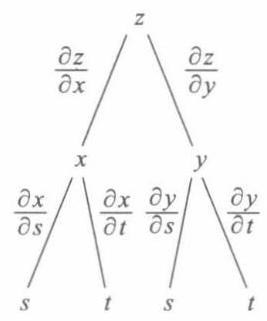
\includegraphics[width=.3\textwidth]{images/P132.jpg}
	\caption{图 $17-5$}
	\label{fig:P132}
\end{figure}

%例 1
\begin{example}

\end{example}
设 \(z = \ln \left( {{u}^{2} + v}\right)\) ,而 \(u = {\mathrm{e}}^{x + {y}^{2}},v = {x}^{2} + y\) ,求
\[
\frac{\partial z}{\partial x},\frac{\partial z}{\partial y}
\]
%解
\begin{solution}

\end{solution}
所讨论的复合函数以 \(x,y\) 为自变量, \(u,v\) 为中间变量. 由于
\[
\frac{\partial z}{\partial u} = \frac{2u}{{u}^{2} + v},\frac{\partial z}{\partial v} = \frac{1}{{u}^{2} + v},
\]
\[
\frac{\partial u}{\partial x} = {\mathrm{e}}^{x + {y}^{2}},\frac{\partial u}{\partial y} = {2y}{\mathrm{e}}^{x + {y}^{2}},\frac{\partial v}{\partial x} = {2x},\frac{\partial v}{\partial y} = 1,
\]
根据公式 (4) 得到
\[
\frac{\partial z}{\partial x} = \frac{\partial z}{\partial u}\frac{\partial u}{\partial x} + \frac{\partial z}{\partial v}\frac{\partial v}{\partial x}
\]
\[
= \frac{2u}{{u}^{2} + v}{\mathrm{e}}^{x + {y}^{2}} + \frac{1}{{u}^{2} + v}{2x} = \frac{2}{{u}^{2} + v}\left( {u{\mathrm{e}}^{x + {y}^{2}} + x}\right) ,
\]
\[
\frac{\partial z}{\partial y} = \frac{\partial z}{\partial u}\frac{\partial u}{\partial y} + \frac{\partial z}{\partial v}\frac{\partial v}{\partial y}
\]
\[
= \frac{2u}{{u}^{2} + v}{2y}{\mathrm{e}}^{x + {y}^{2}} + \frac{1}{{u}^{2} + v} = \frac{1}{{u}^{2} + v}\left( {{4uy}{\mathrm{e}}^{x + {y}^{2}} + 1}\right) .
\]
%例 2
\begin{example}

\end{example}
设 \(u = u\left( {x,y}\right)\) 可微,在极坐标变换 \(x = r\cos \theta ,y = r\sin \theta\) 下,证明:
\[
{\left( \frac{\partial u}{\partial r}\right) }^{2} + \frac{1}{{r}^{2}}{\left( \frac{\partial u}{\partial \theta }\right) }^{2} = {\left( \frac{\partial u}{\partial x}\right) }^{2} + {\left( \frac{\partial u}{\partial y}\right) }^{2}.
\]
%证
\begin{proof}

\end{proof}
\(u\) 可以看作 \(r,\theta\) 的复合函数 \(u = u\left( {r\cos \theta ,r\sin \theta }\right)\) ,因此
\[
\frac{\partial u}{\partial r} = \frac{\partial u}{\partial x}\frac{\partial x}{\partial r} + \frac{\partial u}{\partial y}\frac{\partial y}{\partial r} = \frac{\partial u}{\partial x}\cos \theta  + \frac{\partial u}{\partial y}\sin \theta ,
\]
\[
\frac{\partial u}{\partial \theta } = \frac{\partial u}{\partial x}\frac{\partial x}{\partial \theta } + \frac{\partial u}{\partial y}\frac{\partial y}{\partial \theta } = \frac{\partial u}{\partial x}\left( {-r\sin \theta }\right)  + \frac{\partial u}{\partial y}r\cos \theta .
\]
于是
\[
{\left( \frac{\partial u}{\partial r}\right) }^{2} + \frac{1}{{r}^{2}}{\left( \frac{\partial u}{\partial \theta }\right) }^{2}
\]
\[
= {\left( \frac{\partial u}{\partial x}\cos \theta  + \frac{\partial u}{\partial y}\sin \theta \right) }^{2} + \frac{1}{{r}^{2}}{\left( -\frac{\partial u}{\partial x}r\sin \theta  + \frac{\partial u}{\partial y}r\cos \theta \right) }^{2}
\]
\[
= {\left( \frac{\partial u}{\partial x}\right) }^{2} + {\left( \frac{\partial u}{\partial y}\right) }^{2}.
\]
%例 3
\begin{example}

\end{example}
设 \(z = {uv} + \sin t\) ,其中 \(u = {\mathrm{e}}^{t},v = \cos t\) ,求 \(\frac{\mathrm{d}z}{\mathrm{\;d}t}\) .

%解
\begin{solution}

\end{solution}
根据复合关系, 画出树状图 17-6. 于是
\[
\frac{\mathrm{d}z}{\mathrm{\;d}t} = \frac{\partial z}{\partial u}\frac{\mathrm{d}u}{\mathrm{\;d}t} + \frac{\partial z}{\partial v}\frac{\mathrm{d}v}{\mathrm{\;d}t} + \frac{\partial z}{\partial t}
\]
\[
= v{\mathrm{e}}^{t} + u\left( {-\sin t}\right)  + \cos t
\]
\[
= {\mathrm{e}}^{t}\left( {\cos t - \sin t}\right)  + \cos t.
\]
\begin{figure}
	\centering
	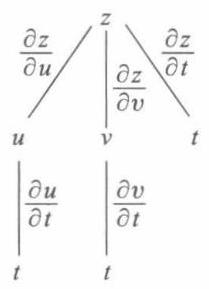
\includegraphics[width=.3\textwidth]{images/P133.jpg}
	\caption{图 $17-6$}
	\label{fig:P133}
\end{figure}

%注
\begin{remark}

\end{remark}
上面第一个等式中,左边的 \(\frac{\mathrm{d}z}{\mathrm{\;d}t}\) 是作为一元函数的复合函数对 \(t\) 求导数,右边最后一项里的 \(\frac{\partial z}{\partial t}\) 是外函数 (作为 \(u,v,t\) 的三元函数) 对 \(t\) 求偏导数,二者所用符号各自有别.

%例 4
\begin{example}

\end{example}
用多元复合微分法计算下列一元函数的导数:

(1) \(y = {x}^{x}\) ;

(2) \(y = \frac{\left( {1 + {x}^{2}}\right) \ln x}{\sin x + \cos x}\) .

%解
\begin{solution}

\end{solution}
(1) 令 \(y = {u}^{v},u = x,v = x\) ,则有
\[
\frac{\mathrm{d}y}{\mathrm{\;d}x} = {y}_{u} \cdot  \frac{\mathrm{d}u}{\mathrm{\;d}x} + {y}_{v} \cdot  \frac{\mathrm{d}v}{\mathrm{\;d}x} = v{u}^{v - 1} + {u}^{v}\ln u
\]
\[
= x \cdot  {x}^{x - 1} + {x}^{x}\ln x = {x}^{x}\left( {1 + \ln x}\right) .
\]
(2)令 \(y = \frac{vw}{u},u = \sin x + \cos x,v = 1 + {x}^{2},w = \ln x\) ,则有
\[
\frac{\mathrm{d}y}{\mathrm{\;d}x} = \frac{\partial y}{\partial u}\frac{\mathrm{d}u}{\mathrm{\;d}x} + \frac{\partial y}{\partial v}\frac{\mathrm{d}v}{\mathrm{\;d}x} + \frac{\partial y}{\partial w}\frac{\mathrm{d}w}{\mathrm{\;d}x}
\]
\[
= \frac{-{vw}}{{u}^{2}}\left( {\cos x - \sin x}\right)  + \frac{w}{u} \cdot  {2x} + \frac{v}{u}\frac{1}{x}
\]
\[
= \frac{1}{{\left( \sin x + \cos x\right) }^{2}}\left\lbrack  {\left( {\sin x + \cos x}\right) \left( {{2x}\ln x + \frac{1 + {x}^{2}}{x}}\right)  - }\right.
\]
\[
\left( {\cos x - \sin x}\right) \left( {1 + {x}^{2}}\right) \ln x\rbrack \text{ . }
\]
由此可见, 以前用 “对数求导法” 求一元函数的导数问题, 如今也可用多元复合函数链式法则来计算.

%例 5
\begin{example}

\end{example}
设 \(u = f\left( {x,y,z}\right) ,y = \varphi \left( {x,t}\right) ,t = \psi \left( {x,z}\right)\) 都有一阶连续偏导数,求 \(\frac{\partial u}{\partial x},\frac{\partial u}{\partial z}\) .

%解
\begin{solution}

\end{solution}
代入中间变量,得到复合函数 \(u = f\left( {x,\varphi \left( {x,\psi \left( {x,z}\right) }\right) ,z}\right)\) 为 \(x,z\) 的函数,参见图 17-7 得到
\[
\frac{\partial u}{\partial x} = \frac{\partial f}{\partial x} + \frac{\partial f}{\partial y}\frac{\partial \varphi }{\partial x} + \frac{\partial f}{\partial y}\frac{\partial \varphi }{\partial t}\frac{\partial \psi }{\partial x};
\]
\[
\frac{\partial u}{\partial z} = \frac{\partial f}{\partial y}\frac{\partial \varphi }{\partial t}\frac{\partial \psi }{\partial z} + \frac{\partial f}{\partial z}.
\]
注意,这里用 \(\frac{\partial u}{\partial x}\) 表示复合函数 \(u = f\left( {x,\varphi \left( {x,\psi \left( {x,z}\right) }\right) ,z}\right)\) 对 \(x\) 的偏导数,而用 \(\frac{\partial f}{\partial x}\) 表示函数 \(u = f\left( {x,y,z}\right)\) 对第一个变量 \(x\) 的偏导数,以区别两者的不同.

%例 6
\begin{example}

\end{example}
设 \(f\left( {x,y}\right)\) 在 \({\mathbf{R}}^{2}\) 上可微,且满足方程: \(y{f}_{x}\left( {x,y}\right)\)  \(= x{f}_{y}\left( {x,y}\right)\) . 证明: 在极坐标中 \(f\) 只是 \(r\) 的函数,即 \(\frac{\partial f}{\partial \theta } = 0\) .

\begin{figure}
	\centering
	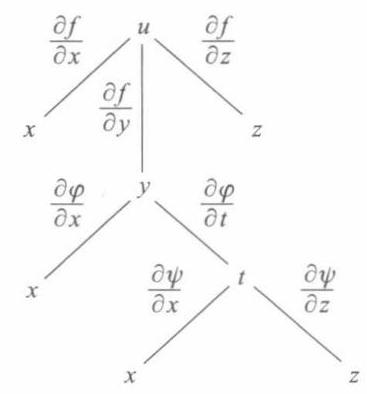
\includegraphics[width=.3\textwidth]{images/P134.jpg}
	\caption{图 $17-7$}
	\label{fig:P134}
\end{figure}

%证
\begin{proof}

\end{proof}
设 \(u = f\left( {x,y}\right) ,x = r\cos \theta ,y = r\sin \theta\) ,则有
\[
\frac{\partial u}{\partial \theta } = \frac{\partial f}{\partial x} \cdot  \frac{\partial x}{\partial \theta } + \frac{\partial f}{\partial y} \cdot  \frac{\partial y}{\partial \theta } = \frac{\partial f}{\partial x} \cdot  \left( {-r\sin \theta }\right)  + \frac{\partial f}{\partial y} \cdot  \left( {r\cos \theta }\right)
\]
\[
=  - y \cdot  \frac{\partial f}{\partial x} + x \cdot  \frac{\partial f}{\partial y} = 0.
\]
\subsection{复合函数的全微分}

若以 \(x\) 和 \(y\) 为自变量的函数 \(z = f\left( {x,y}\right)\) 可微,则其全微分为
\[
\mathrm{d}z = \frac{\partial z}{\partial x}\mathrm{\;d}x + \frac{\partial z}{\partial y}\mathrm{\;d}y. \tag{11}
\]
如果 \(x,y\) 作为中间变量又是自变量 \(s,t\) 的可微函数
\[
x = \varphi \left( {s,t}\right) ,\;y = \psi \left( {s,t}\right) ,
\]
则由定理 17.5 知道,复合函数 \(z = f\left( {\varphi \left( {s,t}\right) ,\psi \left( {s,t}\right) }\right)\) 是可微的,其全微分为
\[
\mathrm{d}z = \frac{\partial z}{\partial s}\mathrm{\;d}s + \frac{\partial z}{\partial t}\mathrm{\;d}t
\]
\[
= \left( {\frac{\partial z}{\partial x}\frac{\partial x}{\partial s} + \frac{\partial z}{\partial y}\frac{\partial y}{\partial s}}\right) \mathrm{d}s + \left( {\frac{\partial z}{\partial x}\frac{\partial x}{\partial t} + \frac{\partial z}{\partial y}\frac{\partial y}{\partial t}}\right) \mathrm{d}t
\]
\[
= \frac{\partial z}{\partial x}\left( {\frac{\partial x}{\partial s}\mathrm{\;d}s + \frac{\partial x}{\partial t}\mathrm{\;d}t}\right)  + \frac{\partial z}{\partial y}\left( {\frac{\partial y}{\partial s}\mathrm{\;d}s + \frac{\partial y}{\partial t}\mathrm{\;d}t}\right) . \tag{12}
\]
由于 \(x,y\) 又是(s, t)的可微函数,因此同时有
\[
\mathrm{d}x = \frac{\partial x}{\partial s}\mathrm{\;d}s + \frac{\partial x}{\partial t}\mathrm{\;d}t,\;\mathrm{\;d}y = \frac{\partial y}{\partial s}\mathrm{\;d}s + \frac{\partial y}{\partial t}\mathrm{\;d}t. \tag{13}
\]
将(13)式代入(12)式,得到与(11)式完全相同的结果. 这就是关于多元函数的一阶 (全) 微分形式不变性.

必须指出,在 (11) 式中当 \(x,y\) 作为自变量时, \(\mathrm{d}x\) 和 \(\mathrm{d}y\) 各自独立取值; 当 \(x,y\) 作为中间变量时, \(\mathrm{d}x\) 和 \(\mathrm{d}y\) 如 (13) 式所示,它们的值由 \(s,t,\mathrm{\;d}s,\mathrm{\;d}t\) 所确定.

利用微分形式不变性, 能更有条理地计算复杂函数的全微分.

%例 7
\begin{example}

\end{example}
设 \(z = {\mathrm{e}}^{xy}\sin \left( {x + y}\right)\) ,利用微分形式不变性求 \(\mathrm{d}z\) ,并由此导出 \(\frac{\partial z}{\partial x}\) 与 \(\frac{\partial z}{\partial y}\) .

%解
\begin{solution}

\end{solution}
令 \(z = {\mathrm{e}}^{u}\sin v,u = {xy},v = x + y\) . 由于
\[
\mathrm{d}z = {z}_{u}\mathrm{\;d}u + {z}_{v}\mathrm{\;d}v = {\mathrm{e}}^{u}\sin v\mathrm{\;d}u + {\mathrm{e}}^{u}\cos v\mathrm{\;d}v,
\]
\[
\mathrm{d}u = y\mathrm{\;d}x + x\mathrm{\;d}y,
\]
\[
\mathrm{d}v = \mathrm{d}x + \mathrm{d}y,
\]
因此
\[
\mathrm{d}z = {\mathrm{e}}^{u}\sin v\left( {y\mathrm{\;d}x + x\mathrm{\;d}y}\right)  + {\mathrm{e}}^{u}\cos v\left( {\mathrm{\;d}x + \mathrm{d}y}\right)
\]
\[
= {\mathrm{e}}^{xy}\left\lbrack  {y\sin \left( {x + y}\right)  + \cos \left( {x + y}\right) }\right\rbrack  \mathrm{d}x +
\]
\[
{\mathrm{e}}^{xy}\left\lbrack  {x\sin \left( {x + y}\right)  + \cos \left( {x + y}\right) }\right\rbrack  \mathrm{d}y,
\]
并由此得到
\[
{z}_{x} = {\mathrm{e}}^{xy}\left\lbrack  {y\sin \left( {x + y}\right)  + \cos \left( {x + y}\right) }\right\rbrack  ,
\]
\[
{z}_{y} = {\mathrm{e}}^{xy}\left\lbrack  {x\sin \left( {x + y}\right)  + \cos \left( {x + y}\right) }\right\rbrack  .
\]
\subsection{习题 17.2}

1. 求下列复合函数的偏导数或导数:

(1)设 \(z = \arctan \left( {xy}\right) ,y = {\mathrm{e}}^{x}\) ,求 \(\frac{\mathrm{d}z}{\mathrm{\;d}x}\) ;

(2)设 \(z = \frac{{x}^{2} + {y}^{2}}{xy}{\mathrm{e}}^{\frac{{x}^{2} + {y}^{2}}{xy}}\) ,求 \(\frac{\partial z}{\partial x},\frac{\partial z}{\partial y}\) ；

(3)设 \(z = {x}^{2} + {xy} + {y}^{2},x = {t}^{2},y = t\) ,求 \(\frac{\mathrm{d}z}{\mathrm{\;d}t}\) ；

(4)设 \(z = {x}^{2}\ln y,x = \frac{u}{v},y = {3u} - {2v}\) ,求 \(\frac{\partial z}{\partial u},\frac{\partial z}{\partial v}\) ;

(5)设 \(u = f\left( {x + y,{xy}}\right)\) ,求 \(\frac{\partial u}{\partial x},\frac{\partial u}{\partial y}\) ；

(6)设 \(u = f\left( {\frac{x}{y},\frac{y}{z}}\right)\) ,求 \(\frac{\partial u}{\partial x},\frac{\partial u}{\partial y},\frac{\partial u}{\partial z}\) .

2. 设 \(z = {\left( x + y\right) }^{xy}\) ,求 \(\mathrm{d}z\) .

3. 设 \(z = \frac{y}{f\left( {{x}^{2} - {y}^{2}}\right) }\) ,其中 \(f\) 为可微函数,验证
\[
\frac{1}{x}\frac{\partial z}{\partial x} + \frac{1}{y}\frac{\partial z}{\partial y} = \frac{z}{{y}^{2}}.
\]
4. 设 \(z = \sin y + f\left( {\sin x - \sin y}\right)\) ,其中 \(f\) 为可微函数,证明
\[
\frac{\partial z}{\partial x}\sec x + \frac{\partial z}{\partial y}\sec y = 1.
\]
5. 设 \(f\left( {x,y}\right)\) 可微,证明: 在坐标旋转变换
\[
x = u\cos \theta  - v\sin \theta ,\;y = u\sin \theta  + v\cos \theta
\]
之下, \({\left( {f}_{x}\right) }^{2} + {\left( {f}_{y}\right) }^{2}\) 是一个形式不变量. 即若
\[
g\left( {u,v}\right)  = f\left( {u\cos \theta  - v\sin \theta ,u\sin \theta  + v\cos \theta }\right) ,
\]
则必有 \({\left( {f}_{x}\right) }^{2} + {\left( {f}_{y}\right) }^{2} = {\left( {g}_{u}\right) }^{2} + {\left( {g}_{v}\right) }^{2}\) (其中旋转角 \(\theta\) 是常数).

6. 设 \(f\left( u\right)\) 是可微函数, \(F\left( {x,t}\right)  = f\left( {x + {2t}}\right)  + f\left( {{3x} - {2t}}\right)\) . 试求:
\[
{F}_{x}\left( {0,0}\right) \text{ 与 }{F}_{t}\left( {0,0}\right) \text{ . }
\]
7. 若函数 \(u = F\left( {x,y,z}\right)\) 满足恒等式 \(F\left( {{tx},{ty},{tz}}\right)  = {t}^{k}F\left( {x,y,z}\right) \left( {t > 0}\right)\) ,则称 \(F\left( {x,y,z}\right)\) 为 \(k\) 次齐次函数. 试证下述关于齐次函数的欧拉定理: 可微函数 \(F\left( {x,y,z}\right)\) 为 \(k\) 次齐次函数的充要条件是
\[
x{F}_{x}\left( {x,y,z}\right)  + y{F}_{y}\left( {x,y,z}\right)  + z{F}_{z}\left( {x,y,z}\right)  = {kF}\left( {x,y,z}\right) .
\]
并证明: \(z = \frac{x{y}^{2}}{\sqrt{{x}^{2} + {y}^{2}}} - {xy}\) 为 2 次齐次函数.

8. 设 \(f\left( {x,y,z}\right)\) 具有性质 \(f\left( {{tx},{t}^{k}y,{t}^{m}z}\right)  = {t}^{n}f\left( {x,y,z}\right) \;\left( {t > 0}\right)\) ,证明:

(1) \(f\left( {x,y,z}\right)  = {x}^{n}f\left( {1,\frac{y}{{x}^{k}},\frac{z}{{x}^{m}}}\right)\) ;



(2) \(x{f}_{x}\left( {x,y,z}\right)  + {ky}{f}_{y}\left( {x,y,z}\right)  + {mz}{f}_{z}\left( {x,y,z}\right)  = {nf}\left( {x,y,z}\right)\) .

9. 设由行列式表示的函数
\[
D\left( t\right)  = \left| \begin{matrix} {a}_{11}\left( t\right) & \cdots & {a}_{1n}\left( t\right) \\  \vdots & & \vdots \\  {a}_{n1}\left( t\right) & \cdots & {a}_{nn}\left( t\right)  \end{matrix}\right| ,
\]
其中 \({a}_{ij}\left( t\right) \;\left( {i,j = 1,2,\cdots ,n}\right)\) 的导数都存在,证明
\[
\frac{\mathrm{d}D\left( t\right) }{\mathrm{d}t} = \mathop{\sum }\limits_{{k = 1}}^{n}\left| \begin{matrix} {a}_{11}\left( t\right) & \cdots & {a}_{1n}\left( t\right) \\  \vdots & & \vdots \\  {a}_{k1}^{\prime }\left( t\right) & \cdots & {a}_{kn}^{\prime }\left( t\right) \\  \vdots & & \vdots \\  {a}_{n1}\left( t\right) & \cdots & {a}_{nn}\left( t\right)  \end{matrix}\right| .
\]
\section{方向导数与梯度}

在许多问题中, 不仅要知道函数在坐标轴方向上的变化率 (即偏导数), 而且还要设法求得函数在其他特定方向上的变化率. 这就是本节所要讨论的方向导数.

%定义  1
\begin{definition}{}{def:}

\end{definition}
设三元函数 \(f\) 在点 \({P}_{0}\left( {{x}_{0},{y}_{0},{z}_{0}}\right)\) 的某邻域 \(U\left( {P}_{0}\right)  \subset  {\mathbf{R}}^{3}\) 有定义, \(l\) 为从点 \({P}_{0}\) 出发的射线, \(P\left( {x,y,z}\right)\) 为 \(l\) 上且含于 \(U\left( {P}_{0}\right)\) 内的任一点,以 \(\rho\) 表示 \(P\) 与 \({P}_{0}\) 两点间的距离. 若极限
\[
\mathop{\lim }\limits_{{\rho  \rightarrow  {0}^{ + }}}\frac{f\left( P\right)  - f\left( {P}_{0}\right) }{\rho } = \mathop{\lim }\limits_{{\rho  \rightarrow  {0}^{ + }}}\frac{{\Delta }_{l}f}{\rho }
\]
存在,则称此极限为函数 \(f\) 在点 \({P}_{0}\) 沿方向 \(l\) 的方向导数,记作
\[
{\left. \frac{\partial f}{\partial \mathbf{l}}\right| }_{{P}_{0}},{f}_{l}\left( {P}_{0}\right) \text{ 或 }{f}_{l}\left( {{x}_{0},{y}_{0},{z}_{0}}\right) .
\]
容易看到,若 \(f\) 在点 \({P}_{0}\) 存在关于 \(x\) 的偏导数,则 \(f\) 在点 \({P}_{0}\) 沿 \(x\) 轴正向的方向导数恰为
\[
{\left. \frac{\partial f}{\partial \mathbf{l}}\right| }_{{P}_{0}} = {\left. \frac{\partial f}{\partial x}\right| }_{{P}_{0}}.
\]
当 \(\mathbf{l}\) 的方向为 \(x\) 轴的负方向时,则有
\[
{\left. \frac{\partial f}{\partial \mathbf{l}}\right| }_{{P}_{0}} =  - {\left. \frac{\partial f}{\partial x}\right| }_{{P}_{0}}.
\]
沿任一方向的方向导数与偏导数的关系由下述定理给出.

%定理 17.6
\begin{theorem}{}{the:}

\end{theorem}
 若函数 \(f\) 在点 \({P}_{0}\left( {{x}_{0},{y}_{0},{z}_{0}}\right)\) 可微,则 \(f\) 在点 \({P}_{0}\) 沿任一方向 \(\mathbf{l}\) 的方向导数都存在, 且
\[
{f}_{l}\left( {P}_{0}\right)  = {f}_{x}\left( {P}_{0}\right) \cos \alpha  + {f}_{y}\left( {P}_{0}\right) \cos \beta  + {f}_{z}\left( {P}_{0}\right) \cos \gamma , \tag{1}
\]
其中 \(\cos \alpha ,\cos \beta ,\cos \gamma\) 为方向 \(l\) 的方向余弦.

%证
\begin{proof}

\end{proof}
设 \(P\left( {x,y,z}\right)\) 为 \(l\) 上任一点,于是 (见图17-8)
\[
\left. \begin{array}{l} x - {x}_{0} = {\Delta x} = \rho \cos \alpha , \\  y - {y}_{0} = {\Delta y} = \rho \cos \beta , \\  z - {z}_{0} = {\Delta z} = \rho \cos \gamma . \end{array}\right\}   \tag{2}
\]
\begin{figure}
	\centering
	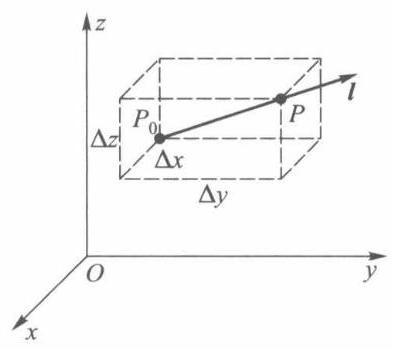
\includegraphics[width=.3\textwidth]{images/P135.jpg}
	\caption{图 $17-8$}
	\label{fig:P135}
\end{figure}

由假设 \(f\) 在点 \({P}_{0}\) 可微,则有
\[
f\left( P\right)  - f\left( {P}_{0}\right)
\]
\[
= {f}_{x}\left( {P}_{0}\right) {\Delta x} + {f}_{y}\left( {P}_{0}\right) {\Delta y} + {f}_{z}\left( {P}_{0}\right) {\Delta z} + o\left( \rho \right) .
\]
上式左、右两边皆除以 \(\rho\) ,并根据 (2) 式可得
\[
\frac{f\left( P\right)  - f\left( {P}_{0}\right) }{\rho } = {f}_{x}\left( {P}_{0}\right) \frac{\Delta x}{\rho } + {f}_{y}\left( {P}_{0}\right) \frac{\Delta y}{\rho } + {f}_{z}\left( {P}_{0}\right) \frac{\Delta z}{\rho } + \frac{o\left( \rho \right) }{\rho }
\]
\[
= {f}_{x}\left( {P}_{0}\right) \cos \alpha  + {f}_{y}\left( {P}_{0}\right) \cos \beta  + {f}_{z}\left( {P}_{0}\right) \cos \gamma  + \frac{o\left( \rho \right) }{\rho }.
\]
因为当 \(\rho  \rightarrow  0\) 时,上式右边末项 \(\frac{o\left( \rho \right) }{\rho } \rightarrow  0\) ,于是左边极限存在且有
\[
{f}_{l}\left( {P}_{0}\right)  = \mathop{\lim }\limits_{{\rho  \rightarrow  {0}^{ + }}}\frac{f\left( P\right)  - f\left( {P}_{0}\right) }{\rho }
\]
\[
= {f}_{x}\left( {P}_{0}\right) \cos \alpha  + {f}_{y}\left( {P}_{0}\right) \cos \beta  + {f}_{z}\left( {P}_{0}\right) \cos \gamma .
\]
对于二元函数 \(f\left( {x,y}\right)\) 来说,相应于 (1) 的结果是
\[
{f}_{l}\left( {P}_{0}\right)  = {f}_{x}\left( {{x}_{0},{y}_{0}}\right) \cos \alpha  + {f}_{y}\left( {{x}_{0},{y}_{0}}\right) \cos \beta ,
\]
其中 \(\alpha ,\beta\) 是平面向量 \(\mathbf{l}\) 的方向角.

%例 1
\begin{example}

\end{example}
设 \(f\left( {x,y,z}\right)  = x + {y}^{2} + {z}^{3}\) ,求 \(f\) 在点 \({P}_{0}\left( {1,1,1}\right)\) 沿方向 \(l : \left( {2, - 2,1}\right)\) 的方向导数.

%解
\begin{solution}

\end{solution}
易见 \(f\) 在点 \({P}_{0}\) 可微. 故由 \({f}_{x}\left( {P}_{0}\right)  = 1,{f}_{y}\left( {P}_{0}\right)  = 2,{f}_{z}\left( {P}_{0}\right)  = 3\) 及方向 \(\mathbf{l}\) 的方向余弦
\[
\cos \alpha  = \frac{2}{\sqrt{{2}^{2} + {\left( -2\right) }^{2} + {1}^{2}}} = \frac{2}{3},
\]
\[
\cos \beta  = \frac{-2}{\sqrt{{2}^{2} + {\left( -2\right) }^{2} + {1}^{2}}} =  - \frac{2}{3},
\]
\[
\cos \gamma  = \frac{1}{\sqrt{{2}^{2} + {\left( -2\right) }^{2} + {1}^{2}}} = \frac{1}{3},
\]
可按公式 (1) 求得 \(f\) 沿方向 \(\mathbf{l}\) 的方向导数为
\[
{f}_{l}\left( {P}_{0}\right)  = 1 \cdot  \frac{2}{3} + 2\left( {-\frac{2}{3}}\right)  + 3 \cdot  \frac{1}{3} = \frac{1}{3}.
\]
%例 2
\begin{example}

\end{example}
设
\[
f\left( {x,y}\right)  = \left\{  \begin{array}{ll} 1, & \text{ 当 }0 < y < {x}^{2}, - \infty  < x <  + \infty \text{ 时, } \\  0, & \text{ 其余部分, } \end{array}\right.
\]
如图 16-8 所示. 这个函数在原点不连续 (当然也不可微), 但在始于原点的任何射线上,都存在包含原点的充分小的一段,在这一段上 \(f\) 的函数值恒为零. 于是由方向导数定义,在原点处沿任何方向 \(\mathbf{l}\) 都有
\[
{\left. \frac{\partial f}{\partial \mathbf{l}}\right| }_{\left( 0,0\right) } = 0.
\]


这个例子说明:(i) 函数在一点可微是方向导数存在的充分条件而不是必要条件. (ii) 函数在一点连续同样不是方向导数存在的必要条件, 当然也不是充分条件 (对此, 读者容易举出反例).

%定义  2
\begin{definition}{}{def:}

\end{definition}
若 \(f\left( {x,y,z}\right)\) 在点 \({P}_{0}\left( {{x}_{0},{y}_{0},{z}_{0}}\right)\) 存在对所有自变量的偏导数,则称向量 \(\left( {{f}_{x}\left( {P}_{0}\right) ,{f}_{y}\left( {P}_{0}\right) ,{f}_{z}\left( {P}_{0}\right) }\right)\) 为函数 \(f\) 在点 \({P}_{0}\) 的梯度,记作\footnote{grad 是英文 gradient(梯度)一词的缩写.}
\[
\operatorname{grad}f = \left( {{f}_{x}\left( {P}_{0}\right) ,{f}_{y}\left( {P}_{0}\right) ,{f}_{z}\left( {P}_{0}\right) }\right) .
\]
向量 \(\operatorname{grad}f\) 的长度 (或模) 为
\[
\left| {\operatorname{grad}f}\right|  = \sqrt{{f}_{x}{\left( {P}_{0}\right) }^{2} + {f}_{y}{\left( {P}_{0}\right) }^{2} + {f}_{z}{\left( {P}_{0}\right) }^{2}}.
\]
在定理 17.6 的条件下,若记 \(\mathbf{l}\) 方向上的单位向量为
\[
{\mathbf{l}}_{0} = \left( {\cos \alpha ,\cos \beta ,\cos \gamma }\right) .
\]
于是方向导数公式又可写成
\[
{f}_{I}\left( {P}_{0}\right)  = \operatorname{grad}f\left( {P}_{0}\right)  \cdot  {\mathbf{l}}_{0} = \left| {\operatorname{grad}f\left( {P}_{0}\right) }\right| \cos \theta ,
\]
这里 \(\theta\) 是梯度向量 \(\operatorname{grad}f\left( {P}_{0}\right)\) 与 \({\mathbf{l}}_{0}\) 的夹角.

因此当 \(\theta  = 0\) 时, \({f}_{l}\left( {P}_{0}\right)\) 取得最大值 \(\left| {\operatorname{grad}f\left( {P}_{0}\right) }\right|\) . 这就是说,当 \(f\) 在点 \({P}_{0}\) 可微时, \(f\) 在点 \({P}_{0}\) 的梯度方向是 \(f\) 的值增长最快的方向,且沿这一方向的变化率就是梯度的模; 而当 \(\mathbf{l}\) 与梯度向量反方向 \(\left( {\theta  = \pi }\right)\) 时,方向导数取得最小值 \(- \left| {\operatorname{grad}f\left( {P}_{0}\right) }\right|\) .

%例 3
\begin{example}

\end{example}
设 \(f\left( {x,y,z}\right)  = x{y}^{2} + y{z}^{3}\) ,求 \(f\) 在 \({P}_{0}\left( {2, - 1,1}\right)\) 的梯度及它的模.

%解
\begin{solution}

\end{solution}
由于 \({f}_{x}\left( {P}_{0}\right)  = 1,{f}_{y}\left( {P}_{0}\right)  =  - 3,{f}_{z}\left( {P}_{0}\right)  =  - 3\) ,所以
\[
\operatorname{grad}f\left( {P}_{0}\right)  = \left( {1, - 3, - 3}\right) ,
\]
\[
\left| {\operatorname{grad}f\left( {P}_{0}\right) }\right|  = \sqrt{{1}^{2} + {\left( -3\right) }^{2} + {\left( -3\right) }^{2}} = \sqrt{19}.
\]
\subsection{习题 17.3}

1. 求函数 \(u = x{y}^{2} + {z}^{3} - {xyz}\) 在点(1,1,2)沿方向 \(l\) (其方向角分别为 \({60}^{ \circ  },{45}^{ \circ  },{60}^{ \circ  }\) ) 的方向导数.

2. 求函数 \(u = {xyz}\) 在沿点 \(A\left( {5,1,2}\right)\) 到点 \(B\left( {9,4,{14}}\right)\) 的方向 \(\overrightarrow{AB}\) 上的方向导数.

3. 求函数 \(u = {x}^{2} + 2{y}^{2} + 3{z}^{2} + {xy} - {4x} + {2y} - {4z}\) 在 \(A = \left( {0,0,0}\right)\) 及 \(B = \left( {5, - 3,\frac{2}{3}}\right)\) 的梯度以及它们的模.

4. 设函数 \(u = \ln \left( \frac{1}{r}\right)\) ,其中 \(r = \sqrt{{\left( x - a\right) }^{2} + {\left( y - b\right) }^{2} + {\left( z - c\right) }^{2}}\) ,求 \(u\) 的梯度,并指出在空间哪些点上成立等式 \(\left| {\operatorname{grad}u}\right|  = 1\) .

5. 设函数 \(u = \frac{{z}^{2}}{{c}^{2}} - \frac{{x}^{2}}{{a}^{2}} - \frac{{y}^{2}}{{b}^{2}}\) ,求它在点(a, b, c)的梯度.

6. 证明:

(1) \(\operatorname{grad}\left( {u + c}\right)  = \operatorname{grad}u\) ( \(c\) 为常数);

 (2) \(\operatorname{grad}\left( {{\alpha u} + {\beta v}}\right)  = \alpha \operatorname{grad}u + \beta \operatorname{grad}v\left( {\alpha ,\beta \text{ 为常数 }}\right)\) ；

( 3 ) grad \(\left( {uv}\right)  = u\) grad \(v + v\) grad \(u\) ;

(4) grad \(f\left( u\right)  = {f}^{\prime }\left( u\right)\) grad \(u\) .

7. 设 \(r = \sqrt{{x}^{2} + {y}^{2} + {z}^{2}}\) ,试求:

(1) grad \(r\) ;

(2) grad \(\frac{1}{r}\) .

8. 设 \(u = {x}^{3} + {y}^{3} + {z}^{3} - {3xyz}\) ,试问在怎样的点集上 \(\operatorname{grad}u\) 分别满足:

(1)垂直于 \(z\) 轴； (2)平行于 \(z\) 轴；

(3)恒为零向量.

9. 设 \(f\left( {x,y}\right)\) 可微, \(l\) 是 \({\mathbf{R}}^{2}\) 上的一个确定向量. 倘若处处有 \({f}_{l}\left( {x,y}\right)  \equiv  0\) ,试问此函数 \(f\) 有何特征?

10. 设 \(f\left( {x,y}\right)\) 可微, \({l}_{1}\) 与 \({l}_{2}\) 是 \({\mathbf{R}}^{2}\) 上的一组线性无关向量. 试证明: 若 \({f}_{{l}_{i}}\left( {x,y}\right)  \equiv  0\left( {i = 1,2}\right)\) ,则 \(f\left( {x,y}\right)  \equiv\) 常数.

\section{泰勒公式与极值问题}

\subsection{高阶偏导数}

由于 \(z = f\left( {x,y}\right)\) 的偏导函数 \({f}_{x}\left( {x,y}\right) ,{f}_{y}\left( {x,y}\right)\) 仍然是自变量 \(x\) 与 \(y\) 的函数,如果它们关于 \(x\) 与 \(y\) 的偏导数也存在,则说函数 \(f\) 具有二阶偏导数,二元函数的二阶偏导数有如下四种情形:
\[
\frac{\partial }{\partial x}\left( \frac{\partial z}{\partial x}\right)  = \frac{{\partial }^{2}z}{\partial {x}^{2}} = {f}_{xx}\left( {x,y}\right) ,
\]
\[
\frac{\partial }{\partial y}\left( \frac{\partial z}{\partial x}\right)  = \frac{{\partial }^{2}z}{\partial x\partial y} = {f}_{xy}\left( {x,y}\right) ,
\]
\[
\frac{\partial }{\partial x}\left( \frac{\partial z}{\partial y}\right)  = \frac{{\partial }^{2}z}{\partial y\partial x} = {f}_{yx}\left( {x,y}\right) ,
\]
\[
\frac{\partial }{\partial y}\left( \frac{\partial z}{\partial y}\right)  = \frac{{\partial }^{2}z}{\partial {y}^{2}} = {f}_{yy}\left( {x,y}\right) .
\]
类似地可定义更高阶的偏导数, \(z = f\left( {x,y}\right)\) 的三阶偏导数共有八种情形,如
\[
\frac{\partial }{\partial x}\left( \frac{{\partial }^{2}z}{\partial {x}^{2}}\right)  = \frac{{\partial }^{3}z}{\partial {x}^{3}} = {f}_{{x}^{3}}\left( {x,y}\right) ,
\]
\[
\frac{\partial }{\partial y}\left( \frac{{\partial }^{2}z}{\partial {x}^{2}}\right)  = \frac{{\partial }^{3}z}{\partial {x}^{2}\partial y} = {f}_{{x}^{2}y}\left( {x,y}\right) ,
\]
............

%例 1
\begin{example}

\end{example}
求函数 \(z = {\mathrm{e}}^{x + {2y}}\) 的所有二阶偏导数和 \(\frac{{\partial }^{3}z}{\partial y\partial {x}^{2}}\) .

%解
\begin{solution}

\end{solution}
由于函数的一阶偏导数是
\[
\frac{\partial z}{\partial x} = {\mathrm{e}}^{x + {2y}},\;\frac{\partial z}{\partial y} = 2{\mathrm{e}}^{x + {2y}}.
\]
因此有
\[
\frac{{\partial }^{2}z}{\partial {x}^{2}} = \frac{\partial }{\partial x}\left( \frac{\partial z}{\partial x}\right)  = \frac{\partial }{\partial x}\left( {\mathrm{e}}^{x + {2y}}\right)  = {\mathrm{e}}^{x + {2y}},
\]
\[
\frac{{\partial }^{2}z}{\partial x\partial y} = \frac{\partial }{\partial y}\left( \frac{\partial z}{\partial x}\right)  = \frac{\partial }{\partial y}\left( {\mathrm{e}}^{x + {2y}}\right)  = 2{\mathrm{e}}^{x + {2y}},
\]

\[
\frac{{\partial }^{2}z}{\partial y\partial x} = \frac{\partial }{\partial x}\left( \frac{\partial z}{\partial y}\right)  = \frac{\partial }{\partial x}\left( {2{\mathrm{e}}^{x + {2y}}}\right)  = 2{\mathrm{e}}^{x + {2y}},
\]
\[
\frac{{\partial }^{2}z}{\partial {y}^{2}} = \frac{\partial }{\partial y}\left( \frac{\partial z}{\partial y}\right)  = \frac{\partial }{\partial y}\left( {2{\mathrm{e}}^{x + {2y}}}\right)  = 4{\mathrm{e}}^{x + {2y}}
\]
和
\[
\frac{{\partial }^{3}z}{\partial y\partial {x}^{2}} = \frac{\partial }{\partial x}\left( \frac{{\partial }^{2}z}{\partial y\partial x}\right)  = \frac{\partial }{\partial x}\left( {2{\mathrm{e}}^{x + {2y}}}\right)  = 2{\mathrm{e}}^{x + {2y}}.
\]
%例 2
\begin{example}

\end{example}
求函数 \(z = \arctan \frac{y}{x}\) 的所有二阶偏导数.

%解
\begin{solution}

\end{solution}
因为 \(\frac{\partial z}{\partial x} = \frac{-y}{{x}^{2} + {y}^{2}},\frac{\partial z}{\partial y} = \frac{x}{{x}^{2} + {y}^{2}}\) ,所以二阶偏导数为
\[
\frac{{\partial }^{2}z}{\partial {x}^{2}} = \frac{\partial }{\partial x}\left( \frac{-y}{{x}^{2} + {y}^{2}}\right)  = \frac{2xy}{{\left( {x}^{2} + {y}^{2}\right) }^{2}},
\]
\[
\frac{{\partial }^{2}z}{\partial x\partial y} = \frac{\partial }{\partial y}\left( \frac{-y}{{x}^{2} + {y}^{2}}\right)  =  - \frac{{x}^{2} - {y}^{2}}{{\left( {x}^{2} + {y}^{2}\right) }^{2}},
\]
\[
\frac{{\partial }^{2}z}{\partial y\partial x} = \frac{\partial }{\partial x}\left( \frac{x}{{x}^{2} + {y}^{2}}\right)  =  - \frac{{x}^{2} - {y}^{2}}{{\left( {x}^{2} + {y}^{2}\right) }^{2}},
\]
\[
\frac{{\partial }^{2}z}{\partial {y}^{2}} = \frac{\partial }{\partial y}\left( \frac{x}{{x}^{2} + {y}^{2}}\right)  = \frac{-{2xy}}{{\left( {x}^{2} + {y}^{2}\right) }^{2}}.
\]
%注
\begin{remark}

\end{remark}
从上面两个例子看到,这些函数关于 \(x\) 和 \(y\) 的不同顺序的两个二阶偏导数都相等 (这种既有关于 \(x\) 又有关于 \(y\) 的高阶偏导数称为混合偏导数),即
\[
\frac{{\partial }^{2}z}{\partial x\partial y} = \frac{{\partial }^{2}z}{\partial y\partial x}.
\]
但这个结论并不对任何函数都成立, 例如函数
\[
f\left( {x,y}\right)  = \left\{  \begin{matrix} {xy}\frac{{x}^{2} - {y}^{2}}{{x}^{2} + {y}^{2}}, & {x}^{2} + {y}^{2} \neq  0, \\  0, & {x}^{2} + {y}^{2} = 0. \end{matrix}\right.
\]
它的一阶偏导数为
\[
{f}_{x}\left( {x,y}\right)  = \left\{  \begin{matrix} \frac{y\left( {{x}^{4} + 4{x}^{2}{y}^{2} - {y}^{4}}\right) }{{\left( {x}^{2} + {y}^{2}\right) }^{2}}, & {x}^{2} + {y}^{2} \neq  0, \\  0, & {x}^{2} + {y}^{2} = 0, \end{matrix}\right.
\]
\[
{f}_{y}\left( {x,y}\right)  = \left\{  \begin{matrix} \frac{x\left( {{x}^{4} - 4{x}^{2}{y}^{2} - {y}^{4}}\right) }{{\left( {x}^{2} + {y}^{2}\right) }^{2}}, & {x}^{2} + {y}^{2} \neq  0, \\  0, & {x}^{2} + {y}^{2} = 0. \end{matrix}\right.
\]
进而求 \(f\) 在(0,0)处关于 \(x\) 和 \(y\) 的两个不同顺序的混合偏导数,得
\[
{f}_{xy}\left( {0,0}\right)  = \mathop{\lim }\limits_{{{\Delta y} \rightarrow  0}}\frac{{f}_{x}\left( {0,{\Delta y}}\right)  - {f}_{x}\left( {0,0}\right) }{\Delta y} = \mathop{\lim }\limits_{{{\Delta y} \rightarrow  0}}\frac{-{\Delta y}}{\Delta y} =  - 1,
\]
\[
{f}_{yx}\left( {0,0}\right)  = \mathop{\lim }\limits_{{{\Delta x} \rightarrow  0}}\frac{{f}_{y}\left( {{\Delta x},0}\right)  - {f}_{y}\left( {0,0}\right) }{\Delta x} = \mathop{\lim }\limits_{{{\Delta x} \rightarrow  0}}\frac{\Delta x}{\Delta x} = 1.
\]
由此看到,这里的 \(f\left( {x,y}\right)\) 在原点处的两个二阶混合偏导数与求导顺序有关. 那么,在什么条件下混合偏导数与求导顺序无关呢? 为此,我们按定义先把 \({f}_{xy}\left( {{x}_{0},{y}_{0}}\right)\) 与 \({f}_{yx}\left( {{x}_{0},{y}_{0}}\right)\) 表示成极限形式. 由于
\[
{f}_{x}\left( {x,y}\right)  = \mathop{\lim }\limits_{{{\Delta x} \rightarrow  0}}\frac{f\left( {x + {\Delta x},y}\right)  - f\left( {x,y}\right) }{\Delta x},
\]
因此有
\[
{f}_{xy}\left( {{x}_{0},{y}_{0}}\right)  = \mathop{\lim }\limits_{{{\Delta y} \rightarrow  0}}\frac{{f}_{x}\left( {{x}_{0},{y}_{0} + {\Delta y}}\right)  - {f}_{x}\left( {{x}_{0},{y}_{0}}\right) }{\Delta y}
\]
\[
= \mathop{\lim }\limits_{{{\Delta y} \rightarrow  0}}\frac{1}{\Delta y}\left\lbrack  {\mathop{\lim }\limits_{{{\Delta x} \rightarrow  0}}\frac{f\left( {{x}_{0} + {\Delta x},{y}_{0} + {\Delta y}}\right)  - f\left( {{x}_{0},{y}_{0} + {\Delta y}}\right) }{\Delta x} - }\right.
\]
\[
\left. {\mathop{\lim }\limits_{{{\Delta x} \rightarrow  0}}\frac{f\left( {{x}_{0} + {\Delta x},{y}_{0}}\right)  - f\left( {{x}_{0},{y}_{0}}\right) }{\Delta x}}\right\rbrack
\]
\[
= \mathop{\lim }\limits_{{{\Delta y} \rightarrow  0}}\mathop{\lim }\limits_{{{\Delta x} \rightarrow  0}}\frac{f\left( {{x}_{0} + {\Delta x},{y}_{0} + {\Delta y}}\right)  - f\left( {{x}_{0},{y}_{0} + {\Delta y}}\right)  - f\left( {{x}_{0} + {\Delta x},{y}_{0}}\right)  + f\left( {{x}_{0},{y}_{0}}\right) }{\Delta x\Delta y}.
\]
(1)

类似地有
\[
{f}_{yx}\left( {{x}_{0},{y}_{0}}\right)
\]
\[
= \mathop{\lim }\limits_{{{\Delta x} \rightarrow  0}}\mathop{\lim }\limits_{{{\Delta y} \rightarrow  0}}\frac{f\left( {{x}_{0} + {\Delta x},{y}_{0} + {\Delta y}}\right)  - f\left( {{x}_{0} + {\Delta x},{y}_{0}}\right)  - f\left( {{x}_{0},{y}_{0} + {\Delta y}}\right)  + f\left( {{x}_{0},{y}_{0}}\right) }{\Delta x\Delta y}.
\]
(2)

为使 \({f}_{xy}\left( {{x}_{0},{y}_{0}}\right)  = {f}_{yx}\left( {{x}_{0},{y}_{0}}\right)\) 成立,必须使 \(\left( 1\right) ,\left( 2\right)\) 这两个累次极限相等,即可以交换累次极限的极限次序. 下述定理给出了使极限 (1), (2) 相等的一个充分条件.

%定理 17.7
\begin{theorem}{}{the:}

\end{theorem}
 若 \({f}_{xy}\left( {x,y}\right)\) 和 \({f}_{yx}\left( {x,y}\right)\) 都在点 \(\left( {{x}_{0},{y}_{0}}\right)\) 连续,则
\[
{f}_{xy}\left( {{x}_{0},{y}_{0}}\right)  = {f}_{yx}\left( {{x}_{0},{y}_{0}}\right) . \tag{3}
\]
%证
\begin{proof}

\end{proof}
令
\[
F\left( {{\Delta x},{\Delta y}}\right)  = f\left( {{x}_{0} + {\Delta x},{y}_{0} + {\Delta y}}\right)  - f\left( {{x}_{0} + {\Delta x},{y}_{0}}\right)  - f\left( {{x}_{0},{y}_{0} + {\Delta y}}\right)  + f\left( {{x}_{0},{y}_{0}}\right) ,
\]
\[
\varphi \left( x\right)  = f\left( {x,{y}_{0} + {\Delta y}}\right)  - f\left( {x,{y}_{0}}\right) .
\]
于是有
\[
F\left( {{\Delta x},{\Delta y}}\right)  = \varphi \left( {{x}_{0} + {\Delta x}}\right)  - \varphi \left( {x}_{0}\right) . \tag{4}
\]
由于函数 \(f\) 存在关于 \(x\) 的偏导数,所以函数 \(\varphi\) 可导. 应用一元函数的中值定理,有
\[
\varphi \left( {{x}_{0} + {\Delta x}}\right)  - \varphi \left( {x}_{0}\right)
\]
\[
= {\varphi }^{\prime }\left( {{x}_{0} + {\theta }_{1}{\Delta x}}\right) {\Delta x}
\]
\[
= \left\lbrack  {{f}_{x}\left( {{x}_{0} + {\theta }_{1}{\Delta x},{y}_{0} + {\Delta y}}\right)  - {f}_{x}\left( {{x}_{0} + {\theta }_{1}{\Delta x},{y}_{0}}\right) }\right\rbrack  {\Delta x}\;\left( {0 < {\theta }_{1} < 1}\right) .
\]
又由 \({f}_{x}\) 存在关于 \(y\) 的偏导数,故对以 \(y\) 为自变量的函数 \({f}_{x}\left( {{x}_{0} + {\theta }_{1}{\Delta x},y}\right)\) 应用一元函数中值定理, 又使上式化为
\[
\varphi \left( {{x}_{0} + {\Delta x}}\right)  - \varphi \left( {x}_{0}\right)  = {f}_{xy}\left( {{x}_{0} + {\theta }_{1}{\Delta x},{y}_{0} + {\theta }_{2}{\Delta y}}\right) {\Delta x\Delta y}\;\left( {0 < {\theta }_{1},{\theta }_{2} < 1}\right) .
\]
由 (4) 则有
\[
F\left( {{\Delta x},{\Delta y}}\right)  = {f}_{xy}\left( {{x}_{0} + {\theta }_{1}{\Delta x},{y}_{0} + {\theta }_{2}{\Delta y}}\right) {\Delta x\Delta y}\;\left( {0 < {\theta }_{1},{\theta }_{2} < 1}\right) . \tag{5}
\]
如果令
\[
\psi \left( y\right)  = f\left( {{x}_{0} + {\Delta x},y}\right)  - f\left( {{x}_{0},y}\right) ,
\]
则有
\[
F\left( {{\Delta x},{\Delta y}}\right)  = \psi \left( {{y}_{0} + {\Delta y}}\right)  - \psi \left( {y}_{0}\right) .
\]
用前面相同的方法, 又可得到
\[
F\left( {{\Delta x},{\Delta y}}\right)  = {f}_{yx}\left( {{x}_{0} + {\theta }_{3}{\Delta x},{y}_{0} + {\theta }_{4}{\Delta y}}\right) {\Delta x\Delta y}\;\left( {0 < {\theta }_{3},{\theta }_{4} < 1}\right) . \tag{6}
\]
当 \({\Delta x},{\Delta y}\) 不为零时,由 (5),(6) 两式得到
\[
{f}_{xy}\left( {{x}_{0} + {\theta }_{1}{\Delta x},{y}_{0} + {\theta }_{2}{\Delta y}}\right)  = {f}_{yx}\left( {{x}_{0} + {\theta }_{3}{\Delta x},{y}_{0} + {\theta }_{4}{\Delta y}}\right) \;\left( {0 < {\theta }_{1},{\theta }_{2},{\theta }_{3},{\theta }_{4} < 1}\right) .
\]
(7)

由定理假设 \({f}_{xy}\left( {x,y}\right)\) 与 \({f}_{yx}\left( {x,y}\right)\) 在点 \(\left( {{x}_{0},{y}_{0}}\right)\) 连续,故当 \({\Delta x} \rightarrow  0,{\Delta y} \rightarrow  0\) 时,(7) 式两边极限都存在而且相等, 这就得到所要证明的 (3) 式.

这个定理的结论对 \(n\) 元函数的混合偏导数也成立. 如三元函数 \(u = f\left( {x,y,z}\right)\) ,若下述六个三阶混合偏导数
\[
{f}_{xyz}\left( {x,y,z}\right) ,\;{f}_{yzx}\left( {x,y,z}\right) ,\;{f}_{zxy}\left( {x,y,z}\right) ,
\]
\[
{f}_{xzy}\left( {x,y,z}\right) ,\;{f}_{yxz}\left( {x,y,z}\right) ,\;{f}_{zyx}\left( {x,y,z}\right)
\]
在某一点都连续,则在这一点六个混合偏导数都相等. 同样,若二元函数 \(z = f\left( {x,y}\right)\) 在点 (x, y)存在直到 \(n\) 阶的连续混合偏导数,则在这一点 \(m\left( { \leq  n}\right)\) 阶混合偏导数都与顺序无关.

今后除特别指出外, 都假设相应阶数的混合偏导数连续, 从而混合偏导数与求导顺序无关.

下面讨论复合函数的高阶偏导数. 设 \(z\) 是通过中间变量 \(x,y\) 而成为 \(s,t\) 的函数,即
\[
z = f\left( {x,y}\right) ,
\]
其中 \(x = \varphi \left( {s,t}\right) ,y = \psi \left( {s,t}\right)\) . 若函数 \(f,\varphi ,\psi\) 都具有连续的二阶偏导数,则作为复合函数的 \(z\) 对 \(s,t\) 同样存在二阶连续偏导数. 具体计算如下:
\[
\frac{\partial z}{\partial s} = \frac{\partial z}{\partial x}\frac{\partial x}{\partial s} + \frac{\partial z}{\partial y}\frac{\partial y}{\partial s},
\]
\[
\frac{\partial z}{\partial t} = \frac{\partial z}{\partial x}\frac{\partial x}{\partial t} + \frac{\partial z}{\partial y}\frac{\partial y}{\partial t}.
\]
显然 \(\frac{\partial z}{\partial s}\) 与 \(\frac{\partial z}{\partial t}\) 仍是 \(s,t\) 的复合函数,其中 \(\frac{\partial z}{\partial x},\frac{\partial z}{\partial y}\) 是 \(x,y\) 的函数, \(\frac{\partial x}{\partial s},\frac{\partial x}{\partial t},\frac{\partial y}{\partial s},\frac{\partial y}{\partial t}\) 是 \(s,t\) 的函数. 继续求 \(z\) 关于 \(s,t\) 的二阶偏导数
\[
\frac{{\partial }^{2}z}{\partial {s}^{2}} = \frac{\partial }{\partial s}\left( \frac{\partial z}{\partial x}\right) \frac{\partial x}{\partial s} + \frac{\partial z}{\partial x} \cdot  \frac{\partial }{\partial s}\left( \frac{\partial x}{\partial s}\right)  + \frac{\partial }{\partial s}\left( \frac{\partial z}{\partial y}\right) \frac{\partial y}{\partial s} + \frac{\partial z}{\partial y} \cdot  \frac{\partial }{\partial s}\left( \frac{\partial y}{\partial s}\right)
\]
\[
= \left( {\frac{{\partial }^{2}z}{\partial {x}^{2}}\frac{\partial x}{\partial s} + \frac{{\partial }^{2}z}{\partial x\partial y}\frac{\partial y}{\partial s}}\right) \frac{\partial x}{\partial s} + \frac{\partial z}{\partial x}\frac{{\partial }^{2}x}{\partial {s}^{2}} + \left( {\frac{{\partial }^{2}z}{\partial y\partial x}\frac{\partial x}{\partial s} + \frac{{\partial }^{2}z}{\partial {y}^{2}}\frac{\partial y}{\partial s}}\right) \frac{\partial y}{\partial s} + \frac{\partial z}{\partial y}\frac{{\partial }^{2}y}{\partial {s}^{2}}
\]
\[
= \frac{{\partial }^{2}z}{\partial {x}^{2}}{\left( \frac{\partial x}{\partial s}\right) }^{2} + 2\frac{{\partial }^{2}z}{\partial x\partial y}\frac{\partial x}{\partial s}\frac{\partial y}{\partial s} + \frac{{\partial }^{2}z}{\partial {y}^{2}}{\left( \frac{\partial y}{\partial s}\right) }^{2} + \frac{\partial z}{\partial x}\frac{{\partial }^{2}x}{\partial {s}^{2}} + \frac{\partial z}{\partial y}\frac{{\partial }^{2}y}{\partial {s}^{2}}.
\]
同理可得
\[
\frac{{\partial }^{2}z}{\partial {t}^{2}} = \frac{{\partial }^{2}z}{\partial {x}^{2}}{\left( \frac{\partial x}{\partial t}\right) }^{2} + 2\frac{{\partial }^{2}z}{\partial x\partial y}\frac{\partial x}{\partial t}\frac{\partial y}{\partial t} + \frac{{\partial }^{2}z}{\partial {y}^{2}}{\left( \frac{\partial y}{\partial t}\right) }^{2} + \frac{\partial z}{\partial x}\frac{{\partial }^{2}x}{\partial {t}^{2}} + \frac{\partial z}{\partial y}\frac{{\partial }^{2}y}{\partial {t}^{2}},
\]
\[
\frac{{\partial }^{2}z}{\partial s\partial t} = \frac{{\partial }^{2}z}{\partial {x}^{2}}\frac{\partial x}{\partial s}\frac{\partial x}{\partial t} + \frac{{\partial }^{2}z}{\partial x\partial y}\left( {\frac{\partial x}{\partial s}\frac{\partial y}{\partial t} + \frac{\partial x}{\partial t}\frac{\partial y}{\partial s}}\right)  + \frac{{\partial }^{2}z}{\partial {y}^{2}}\frac{\partial y}{\partial s}\frac{\partial y}{\partial t} + \frac{\partial z}{\partial x}\frac{{\partial }^{2}x}{\partial s\partial t} + \frac{\partial z}{\partial y}\frac{{\partial }^{2}y}{\partial s\partial t}
\]
\[
= \frac{{\partial }^{2}z}{\partial t\partial s}\text{ . }
\]
%例 3
\begin{example}

\end{example}
设 \(z = f\left( {x,\frac{x}{y}}\right)\) ,求 \(\frac{{\partial }^{2}z}{\partial {x}^{2}},\frac{{\partial }^{2}z}{\partial x\partial y}\) .

%解
\begin{solution}

\end{solution}
这里 \(z\) 是以 \(x\) 和 \(y\) 为自变量的复合函数,它也可改写成如下形式:
\[
z = f\left( {u,v}\right) ,\;u = x,\;v = \frac{x}{y}.
\]
由复合函数求导公式有
\[
\frac{\partial z}{\partial x} = \frac{\partial f}{\partial u}\frac{\partial u}{\partial x} + \frac{\partial f}{\partial v}\frac{\partial v}{\partial x} = \frac{\partial f}{\partial u} + \frac{1}{y}\frac{\partial f}{\partial v}.
\]
注意,这里 \(\frac{\partial f}{\partial u},\frac{\partial f}{\partial v}\) 仍是以 \(u,v\) 为中间变量,以 \(x,y\) 为自变量的复合函数. 所以
\[
\frac{{\partial }^{2}z}{\partial {x}^{2}} = \frac{\partial }{\partial x}\left( {\frac{\partial f}{\partial u} + \frac{1}{y}\frac{\partial f}{\partial v}}\right)
\]
\[
= \frac{{\partial }^{2}f}{\partial {u}^{2}}\frac{\partial u}{\partial x} + \frac{{\partial }^{2}f}{\partial u\partial v}\frac{\partial v}{\partial x} + \frac{1}{y}\left( {\frac{{\partial }^{2}f}{\partial v\partial u}\frac{\partial u}{\partial x} + \frac{{\partial }^{2}f}{\partial {v}^{2}}\frac{\partial v}{\partial x}}\right)
\]
\[
= \frac{{\partial }^{2}f}{\partial {u}^{2}} + \frac{2}{y}\frac{{\partial }^{2}f}{\partial u\partial v} + \frac{1}{{y}^{2}}\frac{{\partial }^{2}f}{\partial {v}^{2}},
\]
\[
\frac{{\partial }^{2}z}{\partial x\partial y} = \frac{\partial }{\partial y}\left( {\frac{\partial f}{\partial u} + \frac{1}{y}\frac{\partial f}{\partial v}}\right)
\]
\[
= \frac{{\partial }^{2}f}{\partial {u}^{2}}\frac{\partial u}{\partial y} + \frac{{\partial }^{2}f}{\partial u\partial v}\frac{\partial v}{\partial y} - \frac{1}{{y}^{2}}\frac{\partial f}{\partial v} + \frac{1}{y}\left( {\frac{{\partial }^{2}f}{\partial v\partial u}\frac{\partial u}{\partial y} + \frac{{\partial }^{2}f}{\partial {v}^{2}}\frac{\partial v}{\partial y}}\right)
\]
\[
=  - \frac{x}{{y}^{2}}\frac{{\partial }^{2}f}{\partial u\partial v} - \frac{x}{{y}^{3}}\frac{{\partial }^{2}f}{\partial {v}^{2}} - \frac{1}{{y}^{2}}\frac{\partial f}{\partial v}\text{ . }
\]
\subsection{中值定理和泰勒公式}

二元函数的中值公式和泰勒公式, 与一元函数的拉格朗日公式和泰勒公式相仿, 对于 \(n\) 元函数 \(\left( {n > 2}\right)\) 也有同样的公式,只是形式上更复杂一些.

在叙述有关定理之前, 先介绍凸区域的概念.

若区域 \(D\) 上任意两点的连线都含于 \(D\) ,则称 \(D\) 为凸区域 (图 17-9). 这就是说,若 \(D\) 为凸区域,则对任意两点 \({P}_{1}\left( {{x}_{1},{y}_{1}}\right) ,{P}_{2}\left( {{x}_{2},{y}_{2}}\right)  \in  D\) 和一切 \(\lambda \left( {0 \leq  \lambda  \leq  1}\right)\) ,恒有
\[
P\left( {{x}_{1} + \lambda \left( {{x}_{2} - {x}_{1}}\right) ,{y}_{1} + \lambda \left( {{y}_{2} - {y}_{1}}\right) }\right)  \in  D.
\]
定理17.8 (中值定理) 设二元函数 \(f\) 在凸开域 \(D \subset  {\mathbf{R}}^{2}\) 上可微,则对任意两点 \(P\left( {a,b}\right) ,Q\left( {a + h,b + k}\right)  \in  D\) ,存在实数 \(\theta \left( {0 < \theta  < 1}\right)\) ,使得
\[
f\left( {a + h,b + k}\right)  - f\left( {a,b}\right)
\]
\[
= {f}_{x}\left( {a + {\theta h},b + {\theta k}}\right) h + {f}_{y}\left( {a + {\theta h},b + {\theta k}}\right) k. \tag{8}
\]
%证
\begin{proof}

\end{proof}
令
\[
\Phi \left( t\right)  = f\left( {a + {th},b + {tk}}\right) .
\]
\begin{figure}
	\centering
	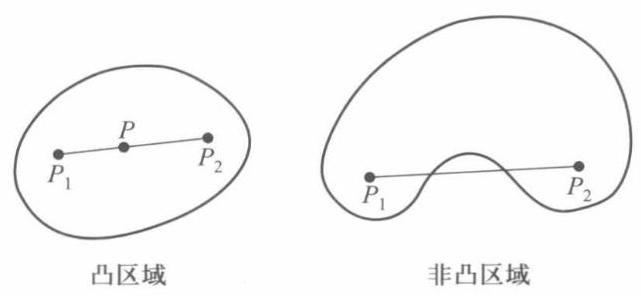
\includegraphics[width=.3\textwidth]{images/P136.jpg}
	\caption{图 $17-9$}
	\label{fig:P136}
\end{figure}

因为 \(D\) 是凸开域,所以 \(\Phi \left( t\right)\) 是定义在 \(\left\lbrack  {0,1}\right\rbrack\) 上的一元函数. 由定理中的条件知 \(\Phi \left( t\right)\) 在 \(\left\lbrack  {0,1}\right\rbrack\) 上连续,在(0,1)上可微. 于是根据一元函数中值定理,存在 \(\theta \left( {0 < \theta  < 1}\right)\) ,使得
\[
\Phi \left( 1\right)  - \Phi \left( 0\right)  = {\Phi }^{\prime }\left( \theta \right) . \tag{9}
\]
由复合函数的求导法则
\[
{\Phi }^{\prime }\left( \theta \right)  = {f}_{x}\left( {a + {\theta h},b + {\theta k}}\right) h + {f}_{y}\left( {a + {\theta h},b + {\theta k}}\right) k. \tag{10}
\]
由于 \(D\) 为凸区域,所以 \(\left( {a + {\theta h},b + {\theta k}}\right)  \in  D\) ,故由 (9),(10) 即得所要证明的 (8) 式.

%注
\begin{remark}

\end{remark}
若 \(D\) 是闭凸域,且对 \(D\) 上任意两点 \({P}_{1}\left( {{x}_{1},{y}_{1}}\right) ,{P}_{2}\left( {{x}_{2},{y}_{2}}\right)\) 及任意 \(\lambda \left( {0 < \lambda  < 1}\right)\) , 都有
\[
P\left( {{x}_{1} + \lambda \left( {{x}_{2} - {x}_{1}}\right) ,{y}_{1} + \lambda \left( {{y}_{2} - {y}_{1}}\right) }\right)  \in  \operatorname{int}D,
\]
则对 \(D\) 上连续, int \(D\) 内可微的函数 \(f\) ,只要 \(P,Q \in  D\) ,也存在 \(\theta  \in  \left( {0,1}\right)\) ,使 (8) 式成立.

例如 \(D\) 是圆域 \(\left\{  {\left( {x,y}\right)  \mid  {\left( x - \xi \right) }^{2} + {\left( y - \eta \right) }^{2} \leq  {r}^{2}}\right\}  ,f\) 在 \(D\) 上连续,在 int \(D\) 内可微,则必有 (8) 式成立. 倘若 \(D\) 是矩形区域 \(\left\lbrack  {a,b}\right\rbrack   \times  \left\lbrack  {c,d}\right\rbrack\) ,那就不能保证对 \(D\) 上任意两点 \(P,Q\) 都有 (8) 式成立 (为什么?).

公式 (8) 也称为二元函数 (在凸域上) 的中值公式. 它与定理 17.3 的中值公式 (12)相比较,差别在于这里的中值点 \(\left( {a + {\theta h},b + {\theta k}}\right)\) 是在 \(P,Q\) 的连线上,而在定理 17.3 中 \({\theta }_{1}\) 与 \({\theta }_{2}\) 可以不相等.

推论 若函数 \(f\) 在区域 \(D\) 上存在偏导数,且
\[
{f}_{x} = {f}_{y} \equiv  0,
\]
则 \(f\) 在区域 \(D\) 上为常量函数.

请读者作为练习自行证明 (注意本推论与 §1 习题 16(2) 两者证明的差别).

%例 4
\begin{example}

\end{example}
对 \(f\left( {x,y}\right)  = \frac{1}{\sqrt{{x}^{2} - {2xy} + 1}}\) 应用微分中值定理,证明存在 \(\theta \left( {0 < \theta  < 1}\right)\) ,使得
\[
1 - \sqrt{2} = \sqrt{2}\left( {1 - {3\theta }}\right) {\left( 1 - 2\theta  + 3{\theta }^{2}\right) }^{-3/2}.
\]
%证
\begin{proof}

\end{proof}
将 \(1 - \sqrt{2} = \sqrt{2}\left( {1 - {3\theta }}\right) {\left( 1 - 2\theta  + 3{\theta }^{2}\right) }^{-3/2}\) 改写成
\[
\frac{1 - \sqrt{2}}{\sqrt{2}} = \left( {1 - {3\theta }}\right) {\left( 1 - 2\theta  + 3{\theta }^{2}\right) }^{-3/2},
\]
左边恰好是 \(f\left( {1,0}\right)  - f\left( {0,1}\right)  = \frac{1}{\sqrt{2}} - 1\) ,所以尝试在凸区域 \(D = \left\{  {\left( {x,y}\right)  \mid  {x}^{2} + {y}^{2} \leq  1}\right\}\) 上,对两点 \({P}_{1}\left( {1,0}\right)\) 与 \({P}_{2}\left( {0,1}\right)\) 应用微分中值定理.

因为当 \({x}^{2} + {y}^{2} \leq  1\) 时, \({x}^{2} - {2xy} + 1 > 0\) ,所以函数 \(f\) 在 \(D\) 上连续,并且
\[
{f}_{x} =  - \frac{x - y}{{\left( {x}^{2} - 2xy + 1\right) }^{3/2}},\;{f}_{y} = \frac{x}{{\left( {x}^{2} - 2xy + 1\right) }^{3/2}}
\]
也在 \(D\) 上连续. \({P}_{1},{P}_{2} \in  D\) ,根据微分中值定理,存在 \(\theta \left( {0 < \theta  < 1}\right)\) ,使得
\[
\frac{1}{\sqrt{2}} - 1 = f\left( {1,0}\right)  - f\left( {0,1}\right)  = {f}_{x}\left( {0 + \theta ,1 - \theta }\right)  \cdot  1 + {f}_{y}\left( {0 + \theta ,1 - \theta }\right)  \cdot  \left( {-1}\right)
\]
\[
=  - \frac{\theta  - \left( {1 - \theta }\right) }{{\left\lbrack  {\theta }^{2} - 2\theta \left( 1 - \theta \right)  + 1\right\rbrack  }^{3/2}} - \frac{\theta }{{\left\lbrack  {\theta }^{2} - 2\theta \left( 1 - \theta \right)  + 1\right\rbrack  }^{3/2}}
\]
\[
= \left( {1 - {3\theta }}\right) {\left( 1 - 2\theta  + 3{\theta }^{2}\right) }^{-3/2}\text{ . }
\]
%定理 17.9
\begin{theorem}{}{the:}

\end{theorem}
 (泰勒定理) 若函数 \(f\) 在点 \({P}_{0}\left( {{x}_{0},{y}_{0}}\right)\) 的某邻域 \(U\left( {P}_{0}\right)\) 上有直到 \(n + 1\) 阶的连续偏导数,则对 \(U\left( {P}_{0}\right)\) 上任一点 \(\left( {{x}_{0} + h,{y}_{0} + k}\right)\) ,存在相应的 \(\theta  \in  \left( {0,1}\right)\) ,使得
\[
f\left( {{x}_{0} + h,{y}_{0} + k}\right)  = f\left( {{x}_{0},{y}_{0}}\right)  + \left( {h\frac{\partial }{\partial x} + k\frac{\partial }{\partial y}}\right) f\left( {{x}_{0},{y}_{0}}\right)  + \frac{1}{2!}{\left( h\frac{\partial }{\partial x} + k\frac{\partial }{\partial y}\right) }^{2}f\left( {{x}_{0},{y}_{0}}\right)  + \cdots  +
\]
\[
\frac{1}{n!}{\left( h\frac{\partial }{\partial x} + k\frac{\partial }{\partial y}\right) }^{n}f\left( {{x}_{0},{y}_{0}}\right)  + \frac{1}{\left( {n + 1}\right) !}{\left( h\frac{\partial }{\partial x} + k\frac{\partial }{\partial y}\right) }^{n + 1}f\left( {{x}_{0} + {\theta h},{y}_{0} + {\theta k}}\right) .
\]
(11)

(11)式称为二元函数 \(f\) 在点 \({P}_{0}\) 的 \(n\) 阶泰勒公式,其中
\[
{\left( h\frac{\partial }{\partial x} + k\frac{\partial }{\partial y}\right) }^{m}f\left( {{x}_{0},{y}_{0}}\right)  = \mathop{\sum }\limits_{{i = 0}}^{m}{\mathrm{C}}_{m}^{i}\frac{{\partial }^{m}}{\partial {x}^{i}\partial {y}^{m - i}}f\left( {{x}_{0},{y}_{0}}\right) {h}^{i}{k}^{m - i}.
\]
%证
\begin{proof}

\end{proof}
与定理 17.8 的证明一样. 作函数
\[
\Phi \left( t\right)  = f\left( {{x}_{0} + {th},{y}_{0} + {tk}}\right) .
\]
由定理的假设,一元函数 \(\Phi \left( t\right)\) 在 \(\left\lbrack  {0,1}\right\rbrack\) 上满足一元函数泰勒定理条件,于是有
\[
\Phi \left( 1\right)  = \Phi \left( 0\right)  + \frac{{\Phi }^{\prime }\left( 0\right) }{1!} + \frac{{\Phi }^{\prime \prime }\left( 0\right) }{2!} + \cdots  + \frac{{\Phi }^{\left( n\right) }\left( 0\right) }{n!} + \frac{{\Phi }^{\left( n + 1\right) }\left( \theta \right) }{\left( {n + 1}\right) !}\;\left( {0 < \theta  < 1}\right) . \tag{12}
\]
应用复合函数求导法则,可求得 \(\Phi \left( t\right)\) 的各阶导数:
\[
{\Phi }^{\left( m\right) }\left( t\right)  = {\left( h\frac{\partial }{\partial x} + k\frac{\partial }{\partial y}\right) }^{m}f\left( {{x}_{0} + {th},{y}_{0} + {tk}}\right) \;\left( {m = 1,2,\cdots ,n + 1}\right) .
\]
当 \(t = 0\) 时,则有
\[
{\Phi }^{\left( m\right) }\left( 0\right)  = {\left( h\frac{\partial }{\partial x} + k\frac{\partial }{\partial y}\right) }^{m}f\left( {{x}_{0},{y}_{0}}\right) \;\left( {m = 1,2,\cdots ,n}\right) , \tag{13}
\]
\[
{\Phi }^{\left( n + 1\right) }\left( \theta \right)  = {\left( h\frac{\partial }{\partial x} + k\frac{\partial }{\partial y}\right) }^{n + 1}f\left( {{x}_{0} + {\theta h},{y}_{0} + {\theta k}}\right) . \tag{14}
\]
将 (13), (14) 式代入 (12) 式就得到所求之泰勒公式 (11).

易见,中值公式 (8) 正是泰勒公式 (11) 在 \(n = 0\) 时的特殊情形.

若在公式 (11) 中只要求余项 \({R}_{n} = o\left( {\rho }^{n}\right) \left( {\rho  = \sqrt{{h}^{2} + {k}^{2}}}\right)\) ,则仅需 \(f\) 在 \(U\left( {P}_{0}\right)\) 内存在直到 \(n\) 阶连续偏导数,便有
\[
f\left( {{x}_{0} + h,{y}_{0} + k}\right)
\]
\[
= f\left( {{x}_{0},{y}_{0}}\right)  + \mathop{\sum }\limits_{{P = 1}}^{n}\frac{1}{P!}{\left( h\frac{\partial }{\partial x} + k\frac{\partial }{\partial y}\right) }^{P}f\left( {{x}_{0},{y}_{0}}\right)  + o\left( {\rho }^{n}\right) . \tag{15}
\]
%例 5
\begin{example}

\end{example}
求 \(f\left( {x,y}\right)  = {x}^{y}\) 在点(1,4)的泰勒公式 (到二阶为止),并用它计算 \({\left( {1.08}\right) }^{3.96}\) .

%解
\begin{solution}

\end{solution}
由于 \({x}_{0} = 1,{y}_{0} = 4,n = 2\) ,因此有
\[
f\left( {x,y}\right)  = {x}^{y},\;f\left( {1,4}\right)  = 1,
\]
\[
{f}_{x}\left( {x,y}\right)  = y{x}^{y - 1},\;{f}_{x}\left( {1,4}\right)  = 4,
\]
\[
{f}_{y}\left( {x,y}\right)  = {x}^{y}\ln x,\;{f}_{y}\left( {1,4}\right)  = 0,
\]
\[
{f}_{{x}^{2}}\left( {x,y}\right)  = y\left( {y - 1}\right) {x}^{y - 2},\;{f}_{{x}^{2}}\left( {1,4}\right)  = {12},
\]
\[
{f}_{xy}\left( {x,y}\right)  = {x}^{y - 1} + y{x}^{y - 1}\ln x,\;{f}_{xy}\left( {1,4}\right)  = 1.
\]
\[
{f}_{{y}^{2}}\left( {x,y}\right)  = {x}^{y}{\left( \ln x\right) }^{2},\;{f}_{{y}^{2}}\left( {1,4}\right)  = 0.
\]
将它们代入泰勒公式(15),即得
\[
{x}^{y} = 1 + 4\left( {x - 1}\right)  + 6{\left( x - 1\right) }^{2} + \left( {x - 1}\right) \left( {y - 4}\right)  + o\left( {\rho }^{2}\right) .
\]
若略去余项,并让 \(x = {1.08},y = {3.96}\) ,则有
\[
{\left( {1.08}\right) }^{3.96} \approx  1 + 4 \times  {0.08} + 6 \times  {0.08}^{2} - {0.08} \times  {0.04} = {1.3552}.
\]
与 §1 例 7 的结果相比较, 这是更接近于精确值 (1.356307...) 的近似值. 因为微分近似式相当于现在的一阶泰勒公式.

\subsection{极值问题}

多元函数的极值问题是多元函数微分学的重要应用, 这里仍以二元函数为例进行讨论.

%定义  1
\begin{definition}{}{def:}

\end{definition}
设函数 \(f\) 在点 \({P}_{0}\left( {{x}_{0},{y}_{0}}\right)\) 的某邻域 \(U\left( {P}_{0}\right)\) 上有定义. 若对于任何点 \(P\left( {x,y}\right)\)  \(\in  U\left( {P}_{0}\right)\) ,成立不等式
\[
\left. {f\left( P\right)  \leq  f\left( {P}_{0}\right) \;\text{ (或 }f\left( P\right)  \geq  f\left( {P}_{0}\right) }\right) ,
\]
则称函数 \(f\) 在点 \({P}_{0}\) 取得极大 (或极小) 值,点 \({P}_{0}\) 称为 \(f\) 的极大 (或极小) 值点. 极大值、 极小值统称极值. 极大值点、极小值点统称极值点.

%注
\begin{remark}

\end{remark}
这里所讨论的极值点只限于定义域的内点.

%例 6
\begin{example}

\end{example}
设 \(f\left( {x,y}\right)  = 2{x}^{2} + {y}^{2},g\left( {x,y}\right)  = \sqrt{1 - {x}^{2} - {y}^{2}},h\left( {x,y}\right)  = {xy}\) . 由定义直接知道,坐标原点(0,0)是 \(f\) 的极小值点,是 \(g\) 的极大值点,但不是 \(h\) 的极值点. 这是因为对任何点 (x, y),恒有 \(f\left( {x,y}\right)  \geq  f\left( {0,0}\right)  = 0\) ; 对任何 \(\left( {x,y}\right)  \in  \left\{  {\left( {x,y}\right)  \mid  {x}^{2} + {y}^{2} \leq  1}\right\}\) ,恒有 \(g\left( {x,y}\right)  \leq\)  \(g\left( {0,0}\right)  = 1\) ; 而对于函数 \(h\) ,在原点的任意小邻域上,既含有使 \(h\left( {x,y}\right)  > 0\) 的 I, III 象限中的点,又含有使 \(h\left( {x,y}\right)  < 0\) 的 II, IV 象限中的点,所以 \(h\left( {0,0}\right)  = 0\) 既不是极大值又不是极小值.

由定义可见,若 \(f\) 在点 \(\left( {{x}_{0},{y}_{0}}\right)\) 取得极值,则当固定 \(y = {y}_{0}\) 时,一元函数 \(f\left( {x,{y}_{0}}\right)\) 必定在 \(x = {x}_{0}\) 取相同的极值. 同理,一元函数 \(f\left( {{x}_{0},y}\right)\) 在 \(y = {y}_{0}\) 也取相同的极值. 于是得到二元函数取极值的必要条件如下:

定理17.10 (极值必要条件) 若函数 \(f\) 在点 \({P}_{0}\left( {{x}_{0},{y}_{0}}\right)\) 存在偏导数,且在 \({P}_{0}\) 取得极值, 则有
\[
{f}_{x}\left( {{x}_{0},{y}_{0}}\right)  = 0,\;{f}_{y}\left( {{x}_{0},{y}_{0}}\right)  = 0. \tag{16}
\]
反之,若函数 \(f\) 在点 \({P}_{0}\) 满足 (16),则称点 \({P}_{0}\) 为 \(f\) 的稳定点. 定理 17.10 指出: 若 \(f\) 存在偏导数,则其极值点必是稳定点. 但稳定点并不都是极值点,如例 6 中的函数 \(h\) ,原点为其稳定点, 但它在原点并不取得极值.

与一元函数的情形相同, 函数在偏导数不存在的点上也有可能取得极值. 例如 \(f\left( {x,y}\right)  = \sqrt{{x}^{2} + {y}^{2}}\) 在原点没有偏导数,但 \(f\left( {0,0}\right)  = 0\) 是 \(f\) 的极小值.

为了讨论二元函数 \(f\) 在点 \({P}_{0}\left( {{x}_{0},{y}_{0}}\right)\) 取得极值的充分条件,我们假定 \(f\) 具有二阶连续偏导数, 并记
\[
{\mathbf{H}}_{f}\left( {P}_{0}\right)  = \left( \begin{array}{ll} {f}_{xx}\left( {P}_{0}\right) & {f}_{xy}\left( {P}_{0}\right) \\  {f}_{yx}\left( {P}_{0}\right) & {f}_{yy}\left( {P}_{0}\right)  \end{array}\right)  = {\left( \begin{array}{ll} {f}_{xx} & {f}_{xy} \\  {f}_{yx} & {f}_{yy} \end{array}\right) }_{{P}_{0}} \tag{17}
\]
它称为 \(f\) 在 \({P}_{0}\) 的黑塞 (Hesse) 矩阵\footnote{关于黑塞矩阵的一般形式,将在第二十三章里介绍.}.

定理17. 11 (极值充分条件) 设二元函数 \(f\) 在点 \({P}_{0}\left( {{x}_{0},{y}_{0}}\right)\) 的某邻域 \(U\left( {P}_{0}\right)\) 上具有二阶连续偏导数,且 \({P}_{0}\) 是 \(f\) 的稳定点. 则当 \({\mathbf{H}}_{f}\left( {P}_{0}\right)\) 是正定矩阵时, \(f\) 在点 \({P}_{0}\) 取得极小值; 当 \({\mathbf{H}}_{f}\left( {P}_{0}\right)\) 是负定矩阵时, \(f\) 在点 \({P}_{0}\) 取得极大值; 当 \({\mathbf{H}}_{f}\left( {P}_{0}\right)\) 是不定矩阵时, \(f\) 在点 \({P}_{0}\) 不取极值.

%证
\begin{proof}

\end{proof}
由 \(f\) 在点 \({P}_{0}\) 的二阶泰勒公式,并注意到条件 \({f}_{x}\left( {P}_{0}\right)  = {f}_{y}\left( {P}_{0}\right)  = 0\) ,有
\[
f\left( {x,y}\right)  - f\left( {{x}_{0},{y}_{0}}\right)
\]
\[
= \frac{1}{2}\left( {{\Delta x},{\Delta y}}\right) {\mathbf{H}}_{f}\left( {P}_{0}\right) {\left( \Delta x,\Delta y\right) }^{\mathrm{T}} + o\left( {\Delta {x}^{2} + \Delta {y}^{2}}\right) .
\]
由于 \({\mathbf{H}}_{f}\left( {P}_{0}\right)\) 正定,所以对任何 \(\left( {{\Delta x},{\Delta y}}\right)  \neq  \left( {0,0}\right)\) ,恒使二次型
\[
Q\left( {{\Delta x},{\Delta y}}\right)  = \left( {{\Delta x},{\Delta y}}\right) {\mathbf{H}}_{f}\left( {P}_{0}\right) {\left( \Delta x,\Delta y\right) }^{\mathrm{T}} > 0.
\]
因此存在一个与 \({\Delta x},{\Delta y}\) 无关的正数 \({q}\)\footnote{因为 \(Q\left( {{\Delta x},{\Delta y}}\right) /\left( {\Delta {x}^{2} + \Delta {y}^{2}}\right)  = \left( {u,v}\right) {\mathbf{H}}_{f}\left( {P}_{0}\right) {\left( u,v\right) }^{\mathrm{T}} = \Phi \left( {u,v}\right)\) ,其中
\[
u = {\Delta x}/\sqrt{\Delta {x}^{2} + \Delta {y}^{2}},\;v = {\Delta y}/\sqrt{\Delta {x}^{2} + \Delta {y}^{2}}.
\]
显然, \(\Phi \left( {u,v}\right)\) 是(u, v)的连续函数. 由于 \({u}^{2} + {v}^{2} = 1\) ,因此 \(\Phi\) 在单位圆 \({u}^{2} + {v}^{2} = 1\) 上必有最小值 \({2q} \geq\) 0 . 又因 \(\left( {u,v}\right)  \neq  \left( {0,0}\right)\) ,故 \(q > 0\) .} ,使得
\[
Q\left( {{\Delta x},{\Delta y}}\right)  \geq  {2q}\left( {\Delta {x}^{2} + \Delta {y}^{2}}\right) .
\]
从而对于充分小的 \(U\left( {P}_{0}\right)\) ,只要 \(\left( {x,y}\right)  \in  U\left( {P}_{0}\right)\) ,就有
\[
f\left( {x,y}\right)  - f\left( {{x}_{0},{y}_{0}}\right)  \geq  q\left( {\Delta {x}^{2} + \Delta {y}^{2}}\right)  + o\left( {\Delta {x}^{2} + \Delta {y}^{2}}\right)
\]
\[
= \left( {\Delta {x}^{2} + \Delta {y}^{2}}\right) \left( {q + o\left( 1\right) }\right)  \geq  0,
\]
即 \(f\) 在点 \(\left( {{x}_{0},{y}_{0}}\right)\) 取得极小值.

同理可证 \({\mathbf{H}}_{f}\left( {P}_{0}\right)\) 为负定矩阵时, \(f\) 在点 \({P}_{0}\) 取得极大值.

最后,当 \({\mathbf{H}}_{f}\left( {P}_{0}\right)\) 不定时, \(f\) 在点 \({P}_{0}\) 不取极值. 这是因为倘若 \(f\) 取极值 (例如取极大值),则沿任何过点 \({P}_{0}\) 的直线 \(x = {x}_{0} + {t\Delta x},y = {y}_{0} + {t\Delta y},f\left( {x,y}\right)  = f\left( {{x}_{0} + {t\Delta x},{y}_{0} + {t\Delta y}}\right)  = \varphi \left( t\right)\) 在 \(t = 0\) 亦取极大值. 由一元函数取极值的充分条件, \({\varphi }^{\prime \prime }\left( 0\right)  > 0\) 是不可能的 (否则 \(\varphi\) 在 \(t\)  \(= 0\) 将取极小值),故 \({\varphi }^{\prime \prime }\left( 0\right)  \leq  0\) . 而
\[
{\varphi }^{\prime }\left( t\right)  = {f}_{x}{\Delta x} + {f}_{y}{\Delta y},
\]
\[
{\varphi }^{\prime \prime }\left( t\right)  = {f}_{xx}\Delta {x}^{2} + 2{f}_{xy}{\Delta x\Delta y} + {f}_{yy}\Delta {y}^{2},
\]
\[
{\varphi }^{\prime \prime }\left( 0\right)  = \left( {{\Delta x},{\Delta y}}\right) {\mathbf{H}}_{f}\left( {P}_{0}\right) {\left( \Delta x,\Delta y\right) }^{\mathrm{T}}.
\]
这表明 \({\mathbf{H}}_{f}\left( {P}_{0}\right)\) 必须是半负定的. 同理,倘若 \(f\) 取极小值,则将导致 \({\mathbf{H}}_{f}\left( {P}_{0}\right)\) 必须是半正

定的. 也就是说,当 \(f\) 在点 \({P}_{0}\) 取得极值时, \({\mathbf{H}}_{f}\left( {P}_{0}\right)\) 必须是半正定或半负定矩阵,但这与假设相矛盾.

根据半正定或半负定对称阵所属主子行列式的符号规则, 定理 17.11 又可写成如下比较实用的形式.

若函数 \(f\) 如定理 17.11 所设. \({P}_{0}\) 是 \(f\) 的稳定点,则有:

(i) 当 \({f}_{xx}\left( {P}_{0}\right)  > 0,\left( {{f}_{xx}{f}_{yy} - {f}_{xy}^{2}}\right) \left( {P}_{0}\right)  > 0\) 时, \(f\) 在点 \({P}_{0}\) 取得极小值;

(ii) 当 \({f}_{xx}\left( {P}_{0}\right)  < 0,\left( {{f}_{xx}{f}_{yy} - {f}_{xy}^{2}}\right) \left( {P}_{0}\right)  > 0\) 时, \(f\) 在点 \({P}_{0}\) 取得极大值;

(iii) 当 \(\left( {{f}_{xx}{f}_{yy} - {f}_{xy}^{2}}\right) \left( {P}_{0}\right)  < 0\) 时, \(f\) 在点 \({P}_{0}\) 不能取得极值;

(iv) 当 \(\left( {{f}_{xx}{f}_{yy} - {f}_{xy}^{2}}\right) \left( {P}_{0}\right)  = 0\) 时,不能肯定 \(f\) 在点 \({P}_{0}\) 是否取得极值.

%例 7
\begin{example}

\end{example}
求 \(f\left( {x,y}\right)  = {x}^{2} + 5{y}^{2} - {6x} + {10y} + 6\) 的极值.

%解
\begin{solution}

\end{solution}
由方程组
\[
\left\{  \begin{array}{l} {f}_{x} = {2x} - 6 = 0, \\  {f}_{y} = {10y} + {10} = 0 \end{array}\right.
\]
得 \(f\) 的稳定点 \({P}_{0}\left( {3, - 1}\right)\) ,由于
\[
{f}_{xx}\left( {P}_{0}\right)  = 2,\;{f}_{xy}\left( {P}_{0}\right)  = 0,
\]
\[
{f}_{yy}\left( {P}_{0}\right)  = {10},\;\left( {{f}_{xx}{f}_{yy} - {f}_{xy}^{2}}\right) \left( {P}_{0}\right)  = {20}.
\]
因此 \(f\) 在点 \({P}_{0}\) 取得极小值 \(f\left( {3, - 1}\right)  =  - 8\) . 又因 \(f\) 处处存在偏导数,故(3, - 1)为 \(f\) 的惟一极值点.

%例 8
\begin{example}

\end{example}
讨论 \(f\left( {x,y}\right)  = {x}^{2} + {xy}\) 是否存在极值.

%解
\begin{solution}

\end{solution}
由方程组 \({f}_{x} = {2x} + y = 0,{f}_{y} = x = 0\) 得稳定点为原点.

因 \({f}_{xx}{f}_{yy} - {f}_{xy}^{2} =  - 1 < 0\) ,故原点不是 \(f\) 的极值点. 又因 \(f\) 处处可微,所以 \(f\) 没有极值点.

%例 9
\begin{example}

\end{example}
讨论 \(f\left( {x,y}\right)  = \left( {y - {x}^{2}}\right) \left( {y - 2{x}^{2}}\right)\) 在原点是否取得极值.

%解
\begin{solution}

\end{solution}
容易验证原点是 \(f\) 的稳定点,且在原点 \({f}_{xx}{f}_{yy} -\)  \({f}_{xy}^{2} = 0\) ,故由定理 17.11 无法判定 \(f\) 在原点是否取到极值. 但由于当 \({x}^{2} < y < 2{x}^{2}\) 时 \(f\left( {x,y}\right)  < 0\) ,而当 \(y > 2{x}^{2}\) 或 \(y < {x}^{2}\) 时, \(f\left( {x,y}\right)  > 0\) (图 17-10),所以函数 \(f\) 不可能在原点取得极值.

\begin{figure}
	\centering
	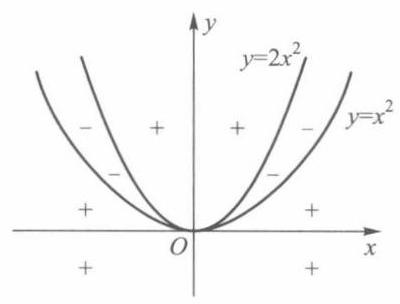
\includegraphics[width=.3\textwidth]{images/P137.jpg}
	\caption{图 $17-10$}
	\label{fig:P137}
\end{figure}

由极值的定义还知道,极值只是函数 \(f\) 在某一点的局部性概念. 要想获得函数 \(f\) 在区域 \(D\) 上的最大值和最小值 (由上一章知道在有界闭区域上的连续函数一定能取得最大与最小值),与一元函数的问题一样,必须考察函数 \(f\) 在所有稳定点、无偏导点以及属于区域的界点上的函数值\footnote{如果属于区域的界点成一曲线 \(F\left( {x,y}\right)  = 0\) ,求函数 \(f\) 在此曲线上的最大 (小) 值一般要用下一章的条件极值方法去解决. 倘若该曲线有一显式方程 \(y = \varphi \left( x\right)\) ,则上述问题归结为求一元函数 \(g\left( x\right)\)  \(= f\left( {x,\varphi \left( x\right) }\right)\) 的极值.}.

比较这些值,其中最大者 (或最小者) 即为函数 \(f\) 在 \(D\) 上的最大 (小) 值.



%例 10
\begin{example}

\end{example}
证明: 圆的所有外切三角形中, 以正三角形的面积为最小.

%证
\begin{proof}

\end{proof}
设圆的半径为 \(a\) . 任一外切三角形为 \(\bigtriangleup {ABC}\) ,三切点处的半径两两相夹的中心角分别为 \(\alpha ,\beta ,\gamma\) . 其中 \(\gamma  = {2\pi } - \left( {\alpha  + \beta }\right)\) (图 17-11). 容易得出 \(\bigtriangleup {ABC}\) 的面积表达式为
\[
S = {a}^{2}\left( {\tan \frac{\alpha }{2} + \tan \frac{\beta }{2} + \tan \frac{\gamma }{2}}\right)
\]
\[
= {a}^{2}\left( {\tan \frac{\alpha }{2} + \tan \frac{\beta }{2} - \tan \frac{\alpha  + \beta }{2}}\right) \text{ . }
\]
\begin{figure}
	\centering
	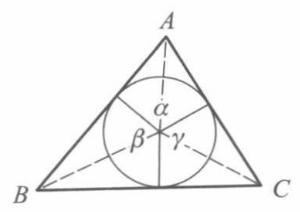
\includegraphics[width=.3\textwidth]{images/P138.jpg}
	\caption{图 $17-11$}
	\label{fig:P138}
\end{figure}

其中 \(0 < \alpha ,\beta  < \pi\) . 为求得稳定点,令
\[
\left\{  \begin{array}{l} {S}_{\alpha } = \frac{1}{2}{a}^{2}\left( {{\sec }^{2}\frac{\alpha }{2} - {\sec }^{2}\frac{\alpha  + \beta }{2}}\right)  = 0, \\  {S}_{\beta } = \frac{1}{2}{a}^{2}\left( {{\sec }^{2}\frac{\beta }{2} - {\sec }^{2}\frac{\alpha  + \beta }{2}}\right)  = 0. \end{array}\right.
\]
在定义域内上述关于 \(\alpha ,\beta\) 的方程组仅有惟一解 \(\alpha  = \beta  = \frac{2}{3}\pi ,\gamma  = {2\pi } - \left( {\alpha  + \beta }\right)  = \frac{2}{3}\pi\) .

为了应用定理 17.11,求得在稳定点 \(\left( {\alpha ,\beta }\right)  = \left( {\frac{2}{3}\pi ,\frac{2}{3}\pi }\right)\) 处的二阶偏导数为
\[
{S}_{\alpha \alpha } = 4\sqrt{3}{a}^{2},{S}_{\alpha \beta } = 2\sqrt{3}{a}^{2},{S}_{\beta \beta } = 4\sqrt{3}{a}^{2}.
\]
由于 \({S}_{\alpha \alpha } > 0,{S}_{\alpha \alpha }{S}_{\beta \beta } - {S}_{\alpha \beta }^{2} = {36}{a}^{4} > 0\) ,因此 \(S\) 在此稳定点上取得极小值.

因为面积函数 \(S\) 在定义域内处处存在偏导数,又因此时 \(\alpha  = \beta  = \gamma\) ,而具体问题存在最小值, 故外切三角形中以正三角形的面积为最小.

%例 11
\begin{example}

\end{example}
(最小二乘法问题) 设通过观测或实验得到一列点 \(\left( {{x}_{i},{y}_{i}}\right) ,i = 1,2,\cdots ,n\) . 它们大体上在一条直线上,即大体上可用直线方程来反映变量 \(x\) 与 \(y\) 之间的对应关系 (参见图 17-12). 现要确定一直线使得与这 \(n\) 个点的偏差平方和最小 (最小二乘方).

\begin{figure}
	\centering
	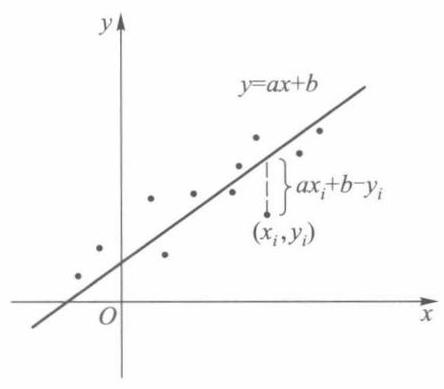
\includegraphics[width=.3\textwidth]{images/P139.jpg}
	\caption{图 $17-12$}
	\label{fig:P139}
\end{figure}

%解
\begin{solution}

\end{solution}
设所求直线方程为
\[
y = {ax} + b,
\]
所测得的 \(n\) 个点为 \(\left( {{x}_{i},{y}_{i}}\right) \left( {i = 1,2,\cdots ,n}\right)\) . 现要确定 \(a,b\) ,使得
\[
f\left( {a,b}\right)  = \mathop{\sum }\limits_{{i = 1}}^{n}{\left( a{x}_{i} + b - {y}_{i}\right) }^{2}
\]
为最小. 为此, 令
\[
\left\{  \begin{array}{l} {f}_{a} = 2\mathop{\sum }\limits_{{i = 1}}^{n}{x}_{i}\left( {a{x}_{i} + b - {y}_{i}}\right)  = 0, \\  {f}_{b} = 2\mathop{\sum }\limits_{{i = 1}}^{n}\left( {a{x}_{i} + b - {y}_{i}}\right)  = 0, \end{array}\right.
\]
把这组关于 \(a,b\) 的线性方程加以整理,得
\[
\left\{  \begin{array}{l} a\mathop{\sum }\limits_{{i = 1}}^{n}{x}_{i}^{2} + b\mathop{\sum }\limits_{{i = 1}}^{n}{x}_{i} = \mathop{\sum }\limits_{{i = 1}}^{n}{x}_{i}{y}_{i}, \\  a\mathop{\sum }\limits_{{i = 1}}^{n}{x}_{i} + {bn} = \mathop{\sum }\limits_{{i = 1}}^{n}{y}_{i}. \end{array}\right.
\]
求此方程组的解,即得 \(f\left( {a,b}\right)\) 的稳定点\footnote{当 \({x}_{1},{x}_{2},\cdots ,{x}_{n}\) 不全相等时,可由数学归纳法证得 \(n\mathop{\sum }\limits_{{i = 1}}^{n}{x}_{i}^{2} - {\left( \mathop{\sum }\limits_{{i = 1}}^{n}{x}_{i}\right) }^{2} > 0\) .}
\[
\bar{a} = \frac{n\mathop{\sum }\limits_{{i = 1}}^{n}{x}_{i}{y}_{i} - \left( {\mathop{\sum }\limits_{{i = 1}}^{n}{x}_{i}}\right) \left( {\mathop{\sum }\limits_{{i = 1}}^{n}{y}_{i}}\right) }{n\mathop{\sum }\limits_{{i = 1}}^{n}{x}_{i}^{2} - {\left( \mathop{\sum }\limits_{{i = 1}}^{n}{x}_{i}\right) }^{2}},
\]
\[
\bar{b} = \frac{\left( {\mathop{\sum }\limits_{{i = 1}}^{n}{x}_{i}^{2}}\right) \left( {\mathop{\sum }\limits_{{i = 1}}^{n}{y}_{i}}\right)  - \left( {\mathop{\sum }\limits_{{i = 1}}^{n}{x}_{i}{y}_{i}}\right) \left( {\mathop{\sum }\limits_{{i = 1}}^{n}{x}_{i}}\right) }{n\mathop{\sum }\limits_{{i = 1}}^{n}{x}_{i}^{2} - {\left( \mathop{\sum }\limits_{{i = 1}}^{n}{x}_{i}\right) }^{2}}.
\]
为进一步确定该点是极小值点, 我们计算得
\[
A = {f}_{aa} = 2\mathop{\sum }\limits_{{i = 1}}^{n}{x}_{i}^{2} > 0,
\]
\[
B = {f}_{ab} = 2\mathop{\sum }\limits_{{i = 1}}^{n}{x}_{i},
\]
\[
C = {f}_{bb} = {2n},
\]
\[
D = {AC} - {B}^{2} = {4n}\mathop{\sum }\limits_{{i = 1}}^{n}{x}_{i}^{2} - 4{\left( \mathop{\sum }\limits_{{i = 1}}^{n}{x}_{i}\right) }^{2} > 0,
\]
从而根据定理 \({17.11},f\left( {a,b}\right)\) 在点 \(\left( {\bar{a},\bar{b}}\right)\) 取得极小值. 由实际问题可知此极小值为最小值.

\subsection{习题 17.4}



\hspace*{2em} 1. 求下列函数的高阶偏导数:

\hspace*{6em} (1) \(z = {x}^{4} + {y}^{4} - 4{x}^{2}{y}^{2}\) ,所有二阶偏导数；

\hspace*{6em} (2) \(z = {\mathrm{e}}^{x}\left( {\cos y + x\sin y}\right)\) ,所有二阶偏导数;

\hspace*{5em} (3) \(z = x\ln \left( {xy}\right) ,\frac{{\partial }^{3}z}{\partial {x}^{2}\partial y},\frac{{\partial }^{3}z}{\partial x\partial {y}^{2}}\) ;

\hspace*{6em} (4) \(u = {xyz}{\mathrm{e}}^{x + y + z},\frac{{\partial }^{p + q + r}u}{\partial {x}^{p}\partial {y}^{q}\partial {z}^{r}}\) ;

\hspace*{6em} (5) \(z = f\left( {x{y}^{2},{x}^{2}y}\right)\) ,所有二阶偏导数;

\hspace*{7em} (6) \(u = f\left( {{x}^{2} + {y}^{2} + {z}^{2}}\right)\) ,所有二阶偏导数;

\hspace*{6em} (7) \(z = f\left( {x + y,{xy},\frac{x}{y}}\right) ,{z}_{x},{z}_{xx},{z}_{xy}\) .

2. 设 \(u = f\left( {x,y}\right) ,x = r\cos \theta ,y = r\sin \theta\) . 证明:




\[
\frac{{\partial }^{2}u}{\partial {r}^{2}} + \frac{1}{r}\frac{\partial u}{\partial r} + \frac{1}{{r}^{2}}\frac{{\partial }^{2}u}{\partial {\theta }^{2}} = \frac{{\partial }^{2}u}{\partial {x}^{2}} + \frac{{\partial }^{2}u}{\partial {y}^{2}}.
\]


\hspace*{4em} 3. 设 \(u = f\left( r\right) ,{r}^{2} = {x}_{1}^{2} + {x}_{2}^{2} + \cdots  + {x}_{n}^{2}\) . 证明:
\[
\frac{{\partial }^{2}u}{\partial {x}_{1}^{2}} + \frac{{\partial }^{2}u}{\partial {x}_{2}^{2}} + \cdots  + \frac{{\partial }^{2}u}{\partial {x}_{n}^{2}} = \frac{{\mathrm{d}}^{2}u}{\mathrm{\;d}{r}^{2}} + \frac{n - 1}{r}\frac{\mathrm{d}u}{\mathrm{\;d}r}.
\]
 4. 设 \(v = \frac{1}{r}g\left( {t - \frac{r}{c}}\right) ,c\) 为常数, \(r = \sqrt{{x}^{2} + {y}^{2} + {z}^{2}}\) . 证明:
\[
{v}_{xx} + {v}_{yy} + {v}_{zz} = \frac{1}{{c}^{2}}{v}_{tt}.
\]
\hspace*{4em} 5. 证明定理 17.8 的推论.

\hspace*{4em} 6. 通过对 \(F\left( {x,y}\right)  = \sin x\cos y\) 施用中值定理,证明对某 \(\theta  \in  \left( {0,1}\right)\) ,有
\[
\frac{3}{4} = \frac{\pi }{3}\cos \frac{\pi \theta }{3}\cos \frac{\pi \theta }{6} - \frac{\pi }{6}\sin \frac{\pi \theta }{3}\sin \frac{\pi \theta }{6}.
\]
 7. 求下列函数在指定点处的泰勒公式:

\hspace*{4em} (1) \(f\left( {x,y}\right)  = \sin \left( {{x}^{2} + {y}^{2}}\right)\) 在点(0,0)(到二阶为止);

\hspace*{4em} (2) \(f\left( {x,y}\right)  = \frac{x}{y}\) 在点(1,1)(到三阶为止);

\hspace*{4em} (3) \(f\left( {x,y}\right)  = \ln \left( {1 + x + y}\right)\) 在点(0,0);

\hspace*{4em} (4) \(f\left( {x,y}\right)  = 2{x}^{2} - {xy} - {y}^{2} - {6x} - {3y} + 5\) 在点(1, - 2).

\hspace*{4em} 8. 求下列函数的极值点:

\hspace*{4em} (1) \(z = {3axy} - {x}^{3} - {y}^{3}\left( {a > 0}\right)\) ;

\hspace*{4em} (2) \(z = {x}^{2} - {xy} + {y}^{2} - {2x} + y\) ;

\hspace*{4em} (3) \(z = {\mathrm{e}}^{2x}\left( {x + {y}^{2} + {2y}}\right)\) .

\hspace*{4em} 9. 求下列函数在指定范围内的最大值与最小值:

\hspace*{4em} (1) \(z = {x}^{2} - {y}^{2},\left\{  {\left( {x,y}\right)  \mid  {x}^{2} + {y}^{2} \leq  4}\right\}\) ;

\hspace*{4em} (2) \(z = {x}^{2} - {xy} + {y}^{2},\{ \left( {x,y}\right) \left| \right| x\left| +\right| y \mid   \leq  1\}\) ;

\hspace*{4em} (3) \(z = \sin x + \sin y - \sin \left( {x + y}\right) ,\{ \left( {x,y}\right)  \mid  x \geq  0,y \geq  0,x + y \leq  {2\pi }\}\) .

\hspace*{4em} 10. 在已知周长为 \({2p}\) 的一切三角形中,求出面积为最大的三角形.

\hspace*{4em} 11. 在 \({xy}\) 平面上求一点,使它到三直线 \(x = 0,y = 0\) 及 \(x + {2y} - {16} = 0\) 的距离平方和最小.

\hspace*{4em} 12. 已知平面上 \(n\) 个点的坐标分别是
\[
{A}_{1}\left( {{x}_{1},{y}_{1}}\right) ,{A}_{2}\left( {{x}_{2},{y}_{2}}\right) ,\cdots ,{A}_{n}\left( {{x}_{n},{y}_{n}}\right) ,
\]
试求一点,使它与这 \(n\) 个点距离的平方和最小.



13. 证明: 函数 \(u = \frac{1}{{2a}\sqrt{\pi t}}{\mathrm{e}}^{-\frac{{\left( x - b\right) }^{2}}{4{a}^{2}t}}\) ( \(a,b\) 为常数) 满足热传导方程
\[
\frac{\partial u}{\partial t} = {a}^{2}\frac{{\partial }^{2}u}{\partial {x}^{2}}.
\]
14. 证明: 函数 \(u = \ln \sqrt{{\left( x - a\right) }^{2} + {\left( y - b\right) }^{2}}\) ( \(a,b\) 为常数) 满足拉普拉斯方程
\[
\frac{{\partial }^{2}u}{\partial {x}^{2}} + \frac{{\partial }^{2}u}{\partial {y}^{2}} = 0.
\]
15. 证明: 若函数 \(u = f\left( {x,y}\right)\) 满足拉普拉斯方程
\[
\frac{{\partial }^{2}u}{\partial {x}^{2}} + \frac{{\partial }^{2}u}{\partial {y}^{2}} = 0,
\]
则函数 \(v = f\left( {\frac{x}{{x}^{2} + {y}^{2}},\frac{y}{{x}^{2} + {y}^{2}}}\right)\) 也满足此方程.

16. 设函数 \(u = \varphi \left( {x + \psi \left( y\right) }\right)\) ,证明
\[
\frac{\partial u}{\partial x}\frac{{\partial }^{2}u}{\partial x\partial y} = \frac{\partial u}{\partial y}\frac{{\partial }^{2}u}{\partial {x}^{2}}.
\]
17. 设 \({f}_{x},{f}_{y}\) 和 \({f}_{yx}\) 在点 \(\left( {{x}_{0},{y}_{0}}\right)\) 的某邻域上存在, \({f}_{yx}\) 在点 \(\left( {{x}_{0},{y}_{0}}\right)\) 连续,证明 \({f}_{xy}\left( {{x}_{0},{y}_{0}}\right)\) 也存在,且 \({f}_{xy}\left( {{x}_{0},{y}_{0}}\right)  = {f}_{yx}\left( {{x}_{0},{y}_{0}}\right) .\)

18. 设 \({f}_{x},{f}_{y}\) 在点 \(\left( {{x}_{0},{y}_{0}}\right)\) 的某邻域上存在且在点 \(\left( {{x}_{0},{y}_{0}}\right)\) 可微,则有
\[
{f}_{xy}\left( {{x}_{0},{y}_{0}}\right)  = {f}_{yx}\left( {{x}_{0},{y}_{0}}\right) .
\]
19. 设
\[
u = \left| \begin{matrix} 1 & 1 & 1 \\  x & y & z \\  {x}^{2} & {y}^{2} & {z}^{2} \end{matrix}\right| .
\]
求:(1) \({u}_{x} + {u}_{y} + {u}_{z}\) ; (2) \(x{u}_{x} + y{u}_{y} + z{u}_{z}\) ; (3) \({u}_{xx} + {u}_{yy} + {u}_{zz}\) .

20. 设 \(f\left( {x,y,z}\right)  = A{x}^{2} + B{y}^{2} + C{z}^{2} + {Dxy} + {Eyz} + {Fzx}\) ,试按 \(h,k,l\) 的正数幂展开 \(f\left( {x + h,y + k,z + l}\right)\) .

\section{总练习题}

1. 设 \(f\left( {x,y,z}\right)  = {x}^{2}y + {y}^{2}z + {z}^{2}x\) ,证明
\[
{f}_{x} + {f}_{y} + {f}_{z} = {\left( x + y + z\right) }^{2}.
\]
2. 求函数
\[
f\left( {x,y}\right)  = \left\{  \begin{matrix} \frac{{x}^{3} - {y}^{3}}{{x}^{2} + {y}^{2}}, & {x}^{2} + {y}^{2} \neq  0, \\  0, & {x}^{2} + {y}^{2} = 0 \end{matrix}\right.
\]
在原点的偏导数 \({f}_{x}\left( {0,0}\right)\) 与 \({f}_{y}\left( {0,0}\right)\) ,并考察 \(f\left( {x,y}\right)\) 在(0,0)的可微性.

3. 设
\[
u = \left| \begin{matrix} 1 & 1 & \cdots & 1 \\  {x}_{1} & {x}_{2} & \cdots & {x}_{n} \\  {x}_{1}^{2} & {x}_{2}^{2} & \cdots & {x}_{n}^{2} \\  \vdots & \vdots & & \vdots \\  {x}_{1}^{n - 1} & {x}_{2}^{n - 1} & \cdots & {x}_{n}^{n - 1} \end{matrix}\right| ,
\]
证明: (1) \(\mathop{\sum }\limits_{{k = 1}}^{n}\frac{\partial u}{\partial {x}_{k}} = 0\) ;

(2) \(\mathop{\sum }\limits_{{k = 1}}^{n}{x}_{k}\frac{\partial u}{\partial {x}_{k}} = \frac{n\left( {n - 1}\right) }{2}u\) .

4. 设函数 \(f\left( {x,y}\right)\) 具有连续的 \(n\) 阶偏导数,试证函数 \(g\left( t\right)  = f\left( {a + {ht},b + {kt}}\right)\) 的 \(n\) 阶导数
\[
\frac{{\mathrm{d}}^{n}g\left( t\right) }{\mathrm{d}{t}^{n}} = {\left( h\frac{\partial }{\partial x} + k\frac{\partial }{\partial y}\right) }^{n}f\left( {a + {ht},b + {kt}}\right) .
\]
5. 设
\[
\varphi \left( {x,y,z}\right)  = \left| \begin{array}{lll} a + x & b + y & c + z \\  d + z & e + x & f + y \\  g + y & h + z & k + x \end{array}\right| ,
\]
求 \(\frac{{\partial }^{2}\varphi }{\partial {x}^{2}}\) .

6. 设
\[
\Phi \left( {x,y,z}\right)  = \left| \begin{array}{lll} {f}_{1}\left( x\right) & {f}_{2}\left( x\right) & {f}_{3}\left( x\right) \\  {g}_{1}\left( y\right) & {g}_{2}\left( y\right) & {g}_{3}\left( y\right) \\  {h}_{1}\left( z\right) & {h}_{2}\left( z\right) & {h}_{3}\left( z\right)  \end{array}\right| ,
\]
求 \(\frac{{\partial }^{3}\Phi }{\partial x\partial y\partial z}\) .

7. 设函数 \(u = f\left( {x,y}\right)\) 在 \({\mathbf{R}}^{2}\) 上有 \({u}_{xy} = 0\) ,试求 \(u\) 关于 \(x,y\) 的函数式.

8. 设 \(f\) 在点 \({P}_{0}\left( {{x}_{0},{y}_{0}}\right)\) 可微,且在 \({P}_{0}\) 给定了 \(n\) 个向量 \({l}_{i},i = 1,2,\cdots ,n\) ,相邻两个向量之间的夹角为 \(\frac{2\pi }{n}\) . 证明
\[
\mathop{\sum }\limits_{{i = 1}}^{n}{f}_{{l}_{i}}\left( {P}_{0}\right)  = 0.
\]
